\documentclass[11pt,a4paper]{report}
\usepackage[utf8]{inputenc} % For UTF-8 encoding
\usepackage[T1]{fontenc}    % For better font encoding
\usepackage[english]{babel} % For English language
\usepackage{graphicx}       % For including images
\usepackage{amsmath,amssymb}% For mathematical symbols
\usepackage{tikz}
\usetikzlibrary{shapes.geometric,arrows,positioning,calc,fit}
\usepackage{hyperref}       % For hyperlinks
\usepackage{geometry}       % For adjusting page margins
\usepackage{fancyhdr}       % For headers and footers
\usepackage{listings}       % For code listings
\usepackage{color}          % For color definitions
\usepackage{caption}        % For customizing captions
\usepackage{booktabs}       % For professional-looking tables
\usepackage{longtable}      % For tables that span multiple pages
\usepackage{float}          % For controlling float positions
\usepackage{array}          % For advanmain ced table options
\usepackage{subfigure}
\usepackage{multirow}
\usepackage{multicol}
\geometry{margin=1in}
\setlength{\parskip}{0.5em}
\setlength{\parindent}{0em}
\usepackage[acronym]{glossaries}
\pagestyle{fancy}
\fancyhf{}
\lhead{Autonomous Driving Car using Modular System Method}
\rhead{\thepage}
\fancypagestyle{noNumber}{%
  \fancyhf{}
  \lhead{Autonomous Driving Car using Modular System Method}
  % clear all
  % no page number here
}
\makeatletter
\let\ps@plain\ps@fancy
\makeatother
\makeglossaries

\newglossaryentry{biodiversity}{
    name=Biodiversity,
    description={The variety of life across all levels of biological organization}
}
\newacronym{cnn}{CNN}{Convolutional Neural Network}
\newacronym{dl}{DL}{Deep Learning}
\newacronym{ml}{ML}{Machine Learning}
\newacronym{vit}{ViT}{Vision Transformers}
\newacronym{iot}{IoT}{Internet of Things}
\newacronym{cv}{CV}{Computer Vision}
\newacronym{mcu}{MCU}{Micro-Controller Unit}
\newacronym{ai}{AI}{Artificial Intelligence}
\renewcommand{\listfigurename}{LIST OF FIGURES}
\renewcommand{\listtablename}{LIST OF TABLES}

% \ifshowcomments
% \newcommand{\mynote}[2]{\fbox{\bfseries\sffamily\scriptsize{#1}}
%  {\small\textsf{\emph{#2}}}}
% %\newcommand{\mynote}[2]{}
% \else
% \newcommand{\mynote}[2]{}
% \fi

% \newcommand{\dq}[1]{\textcolor{red}{\mynote{Quy}{#1}}}
% \newcommand{\hd}[1]{\textcolor{green}{\mynote{Dan}{#1}}}
% \newcommand{\cs}[1]{\textcolor{blue}{\mynote{Cam}{#1}}}



\begin{document}
\pagenumbering{arabic}

\begin{titlepage}
\begin{tikzpicture}[remember picture, overlay]
  \draw[thick] ($(current page.north west) + (2cm, -2cm)$) rectangle ($(current page.south east) + (-2cm, 2cm)$);
\end{tikzpicture}

\begin{center}
    {\small 
    UNIVERSITY OF SCIENCE AND TECHNOLOGY OF HANOI \\
    \textbf{DEPARTMENT OF INFORMATION AND COMMUNICATION TECHNOLOGY} 
    } \\[1.5cm]

    % USTH Logo
    
\includegraphics[width=0.45\linewidth]{/mnt/storage/pylot/report/images/usth.png} \\[1.5cm]

    {\Huge \textbf{BACHELOR THESIS}}\\[1.5cm]

    {\Large By} \\[0.5cm]
    {\Large Nguyen Khanh Linh - 22BA13193} \\[1cm]

    {\Large Title:} \\[0.5cm]
    {\huge \textbf{\uppercase{Autonomous Driving Car using}} \\[0.5cm] 
    \textbf{\uppercase{Modular System Method}}} \\[2cm]
    
    {\Large
    \begin{tabular}{rl}
        Supervisor: & Msc. Le Nhu Chu Hiep \\
    \end{tabular}
    } \\[3cm]

    {\Large \textbf{Hanoi, June -- 2026}}
\end{center}
\end{titlepage}
\clearpage
\pagenumbering{Roman}  % Start Roman page numbering
\setcounter{page}{1}   % Start from I


\tableofcontents
\addcontentsline{toc}{chapter}{Content}
\listoffigures
\addcontentsline{toc}{chapter}{List of Figures}
\clearpage

% List of Tables
\listoftables
\addcontentsline{toc}{chapter}{List of Table}

\printglossary[type=\acronymtype,title=List of Abbreviations]
\addcontentsline{toc}{chapter}{List of Abbreviations}


\chapter*{Declaration}
\addcontentsline{toc}{chapter}{Declartion}
I hereby, Nguyen Khanh Linh, declare that my thesis represents my own work after doing an internship at USTH ICTLAB, University of Science and Technology of Hanoi.

I have read the University’s internship guidelines. In the case of plagiarism appearing in my thesis, I accept responsibility for the conduct of the procedures in accordance with the
University’s Committee.

Hanoi, June 2026\\

Signature\\
\\
\\
\\

Nguyen Khanh Linh


\chapter*{Acknowledgements}
\addcontentsline{toc}{chapter}{Acknowledgements}
 I would like to express my sincere gratitude to Msc. Le Nhu Chu Hiep for his exceptional guidance and support throughout this project. I am also grateful to USTH for providing me with all the resources needed to complete this project and CARLA challenge for creating outstanding simulation system.

\chapter*{Abstract}
\addcontentsline{toc}{chapter}{Abstract}

Autonomous driving systems require the seamless integration of multiple complex software modules, including perception, tracking, prediction, planning, and control, to ensure safe and efficient navigation. Traditionally, end-to-end deep learning approaches suffer from a lack of interpretability and safety guarantees, motivating the industry's preference for modular systems. 

In this thesis, we study and implement a modular autonomous vehicle pipeline using Pylot, an open-source autonomous driving platform built on top of the ERDOS dataflow framework, and evaluate its performance in the CARLA simulator. We address the challenge of modular system integration and component evaluation. The main contributions of this thesis include:
\begin{itemize}
    \item Deploying and configuring the Pylot modular autonomous driving stack on the CARLA simulator.
    \item Training a custom YOLOv8 object detector for real-time 2D/3D obstacle detection to replace missing baseline models, and benchmarking it against ground-truth simulator perception.
    \item Integrating classical computer vision techniques, specifically HSV color space thresholding and the Hough Transform, for efficient and robust lane detection.
    \item Integrating the perception system with a SORT tracking operator and a linear trajectory prediction module to predict obstacle futures.
    \item Running closed-loop simulation tests with Waypoint-based planning and PID control to evaluate driving safety under varying scenario conditions.
\end{itemize}

The experimental results show that the modular approach enables rapid debugging and evaluation of individual components, demonstrating that our custom YOLOv8 model combined with the PID controller successfully navigates target paths while maintaining safety boundaries.

\textbf{Keywords:} Autonomous Driving, CARLA Simulator, Modular Systems, ERDOS, YOLOv8, Obstacle Tracking, Waypoint Planning.

\clearpage
\pagenumbering{arabic}
\setcounter{page}{1}
\chapter{Introduction}
\section{Context and motivation}
\label{sec:context}
\subsection{Context}
In the 90s, after cars were invented and became popular for every household, science fiction books and movies were trying to illustrate how a car could operate by itself in the far future. Nowadays, with significant improvements in Computer Science, Machine Learning and Deep Learning, humans are making the dream come true. From the simplest neural network for road segmentation called ALVINN (Autonomous Land Vehicle In a Neural Network)~\cite{alvinn1989} by Dean A. Pomerleau, Autonomous vehicles (AVs) have developed from movie magic to fully functional autonomous vehicles, driven by innovation in computer vision, deep learning, and robotic control. However, deploying safe, reliable and fully automatic autonomous driving software on physical vehicles remains extremely challenging due to safety-critical constraints, dynamic environments, and the need for real-time processing.

Two main approaches for Autonomous driving architectures are end-to-end approaches and modular pipelines. While end-to-end deep learning maps sensor inputs directly to a single program which is responsible for sticking to lanes, detecting surroundings, making decisions, handling surprise situations and controlling vehicles, it lacks explainability and safety guarantees. A modular system pipeline divides the load to multiple sequential tasks:
\begin{enumerate}
    \item \textbf{Perception:} Converting raw sensor inputs (camera, LiDAR, GPS) into structured representations of the environment.
    \item \textbf{Tracking:} Keep track of detected obstacles across time frames.
    \item \textbf{Prediction:} Predict the future trajectory of other agents.
    \item \textbf{Planning:} Computing a safe, clear route to the destination.
    \item \textbf{Control:} Generating physical actuation (steering, throttle, brake) to execute the planned trajectory.
\end{enumerate}

Developing and testing these modules on real vehicles (such as the Lincoln MKZ) is expensive and highly risky. Thus, high-fidelity simulators like CARLA have become standard for evaluating modular stacks under diverse traffic scenarios.

\subsection{Problem Statement}
In a modular autonomous driving stack, the overall safety and efficiency of the ego-vehicle (The vehicle the pipeline controlling) are heavily dependent on the performance of individual modules and their interactions. A major problem in such systems is error propagation: a failure in the perception module (e.g., misdetecting a pedestrian or a traffic light) propagates through tracking, prediction, and planning, eventually leading to a critical failure in control (e.g., a collision). Furthermore, coordinating these modules in real-time requires a highly efficient dataflow framework that minimizes latency, manages data synchronization, and ensures smooth execution.

\subsection{Motivation}
This research is motivated by the need to understand, build, and evaluate a robust, modular autonomous driving pipeline. Using Pylot — a platform that relies on the ERDOS dataflow system, which allows us to build a graph of operators where data-stream flow asynchronously and accurately. By utilizing CARLA, we can test the modular pipeline under identical environmental conditions, analyze the trade-offs of running perfect (ground-truth) vs. visual-perception-based modules (such as YOLOv8 obstacle detection), and evaluate the overall driving results.

\section{Related Work}
\label{sec:related_work}
The development of autonomous driving systems has sped up drastically within several decades. Early efforts in the 1980s, such as the Carnegie Mellon Navlab~\cite{thorpe1988} and the VaMP system~\cite{dickmanns1994, dickmanns1986}, relied on traditional computer vision and early control strategies. Pomerleau's ALVINN~\cite{alvinn1989} demonstrated one of the first uses of neural networks for road following.

Modern autonomous driving architectures can largely be divided into modular and end-to-end approaches. The modular paradigm separates the driving task into discrete components like perception, planning, and control~\cite{wang2023}. In perception, advancements in deep learning models such as AlexNet~\cite{alexnet2012}, ResNet~\cite{resnet2016}, and YOLO~\cite{yolo2016} have provided excellent real-time object detection, while 3D perception has advanced with methods like MV3D~\cite{mv3d2017}. The nuScenes dataset~\cite{nuscenes2020} has further standardized the evaluation of these modular components.

In addition, end-to-end driving models by Bojarski et al.~\cite{bojarski2016} and Levine et al.~\cite{levine2016} train a single neural network to map raw sensor inputs directly to control commands~\cite{xu2017}. While these methods have found ways to incorporate deep reinforcement learning~\cite{aradi2020} and vision transformers~\cite{swin2021}, they face challenges with interpretability~\cite{bojarski2019} and suffer from limitations in behavior cloning~\cite{codevilla2019}.

Recent works have found ways to improve planning-oriented models like UniAD~\cite{uniad2023} and the deployment of Foundation Models~\cite{wu2025}. Our work builds upon the reliable modular architecture standard, using the Pylot framework~\cite{erdos_pylot} to integrate a custom YOLO detection pipeline.

\section{Thesis Objective} 
\label{sec: obj}
The primary objective of this thesis is to implement, integrate, and evaluate a modular autonomous driving car system using the Pylot framework on top of the CARLA simulator. Due to the unavailability of original baseline detection models, a critical objective is to collect data from CARLA, train a custom YOLOv8 model for obstacle detection, and evaluate its impact on the downstream tracking, planning, and control modules. Furthermore, this thesis aims to integrate classical computer vision methodologies, namely HSV color space thresholding and the Hough Transform, to establish a robust and low-latency lane detection pipeline. The performance of the modular stack is benchmarked against perfect perception configs to assess the limits of visual perception in closed-loop driving scenarios.

\section{Thesis Structure}
\label{sec: structure}
The remainder of this thesis is structured as follows:
\begin{itemize}
    \item \textbf{Chapter 1} introduces the context, modular architecture, problem statement, and objective of this research.
    \item \textbf{Chapter 2} discusses the technical background of Pylot, the ERDOS framework, the CARLA simulator, and individual components such as YOLOv8, SORT, and PID control.
    \item \textbf{Chapter 3} details the methodology, including data collection, custom YOLOv8 model training, dataflow graph construction, and component integration.
    \item \textbf{Chapter 4} describes the experimental setup, scenario benchmarks, and performance evaluation of both visual-perception and ground-truth pipelines.
    \item \textbf{Chapter 5} summarizes the findings of this thesis and outlines future avenues of research.
\end{itemize}



\chapter{Background}

This chapter introduces the general information of the Pylot autonomous vehicle stack and its components. Pylot is built on top of the ERDOS dataflow system and executes inside the CARLA simulation environment. The core modules of the pipeline include perception, tracking, prediction, planning, and control.


\section{Autonomous Driving Architectures}
\label{sec:architectures}
Autonomous driving systems typically follow either an end-to-end learning paradigm or a modular system architecture. 
Modular system architectures break down the autonomous driving pipeline into specialized modules such as perception, tracking, prediction, planning, and control. This design has become the industry standard because it provides safety guarantees while providing ground-truth information to asset the pipeline performance, as well as allows independent verification and validation of each component. 

Pylot~\cite{erdos_pylot} is a modular autonomous vehicle platform designed for developing and testing these individual components. It utilizes the ERDOS dataflow engine to model the autonomous driving pipeline as a directed graph of operators connected by data streams.

\subsection{ERDOS Dataflow Engine}
In modular autonomous vehicle pipeline, latency and data synchronization are crucial. Autonomous vehicles generate high-frequency sensor streams (e.g., cameras at 30 Hz, LiDAR at 10 Hz), and processing operators have varying runtimes. Connecting these operators requires a system that manages latency and consistency.

ERDOS addresses these challenges using a dataflow paradigm. In ERDOS, each component is implemented as an \textit{operator} that receives data via input streams and publishes data to output streams. Streams contain data, timestamps, and watermarks:
\begin{itemize}
    \item \textbf{Timestamps}: Indicate the simulated or real-world time at which the sensor data was captured.
    \item \textbf{Watermarks}: A control message indicating that no further messages with a timestamp less than or equal to the watermark will be sent on that stream. Operators use watermarks to safely process data, ensuring that downstream planners and controllers do not act on incomplete or out-of-order perception data.
\end{itemize}

\subsubsection{Comparison with Traditional Middlewares}
Most contemporary autonomous vehicles rely on the Robot Operating System (ROS) as their primary middleware. ROS 1 utilizes a loosely coupled publisher-subscriber model with a centralized master node (roscore) and communicates via TCP/UDP sockets. While flexible, this model introduces significant serialization and deserialization overhead, which severely bottlenecks high-frequency, high-bandwidth sensor streams such as camera captures traffic jams or dense LiDAR point clouds. ROS 2 attempted to rectify this by migrating to the Data Distribution Service (DDS) standard, offering Quality of Service (QoS) policies, but it still struggles with decisive execution. In ROS, a node receiving data from multiple sensors at different frequencies (e.g., a 30 Hz camera and a 10 Hz LiDAR) must manually manage message synchronization policies (e.g., \texttt{message\_filters} in ROS), which often leads to dropped messages or processing of temporally misaligned data.

To tackle this problem, ERDOS mitigates these hardware and synchronization bottlenecks through zero-copy communication. When two ERDOS operators reside on the same physical machine, they exchange data by passing pointers to shared memory regions, entirely bypassing the network stack and serialization overhead. Furthermore, the watermark-driven execution model inherently reduces the autonomous driving pipeline to a Kahn Process Network (KPN)~\cite{kahn_process}. In a KPN, operators are deterministic sequential processes that communicate exclusively through unbounded FIFO channels. Because execution is strictly gated by the arrival of watermarks, ERDOS guarantees that the autonomous vehicle will produce the exact same sequence of actuation commands given the same sequence of sensor inputs, regardless of operating system thread scheduling or hardware load. This output-determinism is invaluable for reproducing edge-case crashes and systematically debugging the latency-accuracy tradeoff.

\subsection{CARLA Simulator Architecture}
Testing modular stacks on physical cars is expensive and dangerous. The CARLA simulator~\cite{carla_sim} is an open-source, high-quality urban driving simulator built on Unreal Engine 4 (UE4). CARLA provides a simulated physics engine, realistic weather and lighting conditions, dynamic obstacles (vehicles, pedestrians), and detailed maps (Town01 through Town05, etc.) containing lanes, traffic lights, and road layouts. 

CARLA is engineered around a scalable client-server architecture. The server is responsible for rendering the 3D environment, computing the rigid body physics of the vehicles, updating the behavior of non-player characters (NPCs) via the Traffic Manager, and computing the intersections of sensor raycasts. The client (in this case, the Pylot framework) connects to the server via a TCP/IP API to retrieve sensor data and dispatch control commands. 

\subsubsection{Synchronous and Asynchronous Execution}
A critical feature of CARLA for modular pipeline evaluation is its dual execution modes. In \textbf{Asynchronous mode}, the CARLA server runs as fast as possible or at a fixed time-step, completely independent of the client. If the client's perception neural networks take too long to process a frame, the server will continue to advance the physics simulation, causing the client's control commands to be applied late. This realistically simulates hardware latency on a physical vehicle. Conversely, in \textbf{Synchronous mode}, the server waits for a "tick" command from the client before computing the next simulation step. Synchronous mode is crucial for generating pristine training datasets and for isolating algorithmic accuracy from hardware latency.

\subsubsection{Sensor Suite and OpenDRIVE Maps}
Pylot interfaces directly with CARLA's extensive sensor suite. The RGB cameras simulate real-world optical properties including field of view (FOV), motion blur, and lens distortion. The LiDAR sensor simulates a rotating array of lasers using raycasting against the UE4 scene geometry, returning a 3D point cloud parameterized by rotation frequency, number of channels, and upper/lower FOV limits. Furthermore, CARLA environments are strictly grounded in the ASAM OpenDRIVE standard. OpenDRIVE provides an XML-based topological representation of the road network, defining lane geometries, junction interconnects, and traffic signal locations. Pylot parses this OpenDRIVE data to construct its internal HD Map, which is heavily utilized by the route and behavioral planning modules to compute legal traversal paths.

\section{Perception Module}
\label{sec:perception}
The perception module is the initial stage of the modular autonomous driving stack. According to the Pylot paper~\cite{erdos_pylot}, this component comprises operators that process camera and LiDAR data to detect and localize objects, lanes, and traffic lights. These operators communicate their results via an \texttt{ObstacleMessage} that contains the bounding box of the detected object along with the confidence score returned by the ML model.
\begin{itemize}
    \item \textbf{Role}: To interpret raw sensor data from the environment and output structured, localized descriptions of obstacles (bounding boxes).
    \item \textbf{Inputs}: Raw camera images (RGB), depth maps (for 3D coordinate projection), and camera calibration parameters (intrinsic and extrinsic matrices).
    \item \textbf{Outputs}: 2D bounding boxes projected into 3D camera/world coordinates with class labels (e.g., vehicle, pedestrian) and detection confidence scores.
\end{itemize}
In Pylot, three main object detection models are supported or discussed as potential backends: Faster R-CNN, EfficientDet, and YOLOv8.

\subsection{Faster R-CNN}
Faster R-CNN~\cite{faster_rcnn} is a classic two-stage object detection model. The first stage consists of a Feature Pyramid Network (FPN) and a Region Proposal Network (RPN) that proposes potential bounding box locations (regions of interest, RoIs). RPN is anchor-based, evaluating potential boxes of multiple scales and aspect ratios at each feature map grid cell. RPN minimizes a multi-task loss containing a binary classification loss (whether an object is present or not) and a bounding box regression loss:
\begin{equation}
    \mathcal{L}_{\text{RPN}}(\{p_i\}, \{t_i\}) = \frac{1}{N_{\text{cls}}} \sum_i \mathcal{L}_{\text{cls}}(p_i, p_i^*) + \lambda \frac{1}{N_{\text{reg}}} \sum_i p_i^* \mathcal{L}_{\text{reg}}(t_i, t_i^*)
\end{equation}
where $p_i$ is the predicted probability of anchor $i$ being an object, $p_i^*$ is the ground-truth label, $t_i$ is the vector representing predicted parameterized coordinates, and $t_i^*$ is the ground-truth coordinates. The second stage crops features from these regions using RoI pooling or RoIAlign and passes them through a fully connected classifier head to predict final class labels and refine the bounding box boundaries via Smooth-$L_1$ loss. Faster R-CNN achieves high localization accuracy but suffers from high computational latency, making it less suitable for real-time edge execution without substantial GPU acceleration.

\subsection{EfficientDet}
EfficientDet~\cite{efficientdet} is a single-stage object detector designed by Google. It introduces a weighted bi-directional feature pyramid network (BiFPN) and a compound scaling method that uniformly scales the depth, width, and resolution of the backbone, feature network, and box/class prediction networks. Standard FPNs treat input features equally regardless of resolution, but BiFPN introduces learnable weights to allow the network to learn the importance of different input features:
\begin{equation}
    O = \sum_i \frac{w_i \cdot I_i}{\epsilon + \sum_j w_j}
\end{equation}
where $I_i$ are the input features, $w_i \ge 0$ are learnable weights, and $\epsilon$ is a small scalar to prevent division by zero. EfficientDet achieves high efficiency across a range of resource constraints, balancing latency and detection mean Average Precision (mAP) through its scaled variants (D0 to D7).

\subsection{YOLOv8}
YOLOv8~\cite{yolov8} is a state-of-the-art single-stage object detector developed by Ultralytics. Unlike Faster R-CNN, YOLOv8 treats object detection as a single regression problem, predicting bounding boxes and class probabilities directly from full images in a single forward pass. YOLOv8 utilizes an anchor-free design with a decoupled head, separating classification and regression tasks, as illustrated in Figure~\ref{fig:yolov8_arch}.

\subsubsection{Backbone and Neck Architecture}
The feature extraction backbone of YOLOv8 is an enhanced version of CSPDarknet53 (Cross Stage Partial Network). The CSP architecture partitions the feature map of the base layer into two parts and then merges them through a cross-stage hierarchy. This reduces the amount of computation and memory overhead while ensuring that the network learns rich gradient flow information. To capture spatial hierarchies at multiple scales, YOLOv8 employs a Spatial Pyramid Pooling - Fast (SPPF) module at the end of the backbone, which pools features using varying receptive fields (kernel sizes $5 \times 5, 9 \times 9, 13 \times 13$). 

The neck of the network utilizes a Path Aggregation Network (PANet) topology. While traditional FPNs only pass semantic information top-down, PANet introduces an additional bottom-up path augmentation. This bidirectional flow ensures that strong localization features from lower layers are efficiently propagated to the higher semantic layers, which is absolutely critical for accurately detecting small obstacles like pedestrians at long distances in the CARLA simulator.

\subsubsection{Data Augmentation Strategies}
To ensure the robustness of the YOLOv8 detector within the CARLA environment, extensive data augmentation strategies are employed during training. The best technique is \textbf{Mosaic Augmentation}, which combines four distinct training images into a single composite mosaic. This drastically increases the variance of object scales and contexts within a single batch, forcing the model to learn scale-invariant features. Furthermore, it naturally mitigates the class imbalance problem by combining images with sparse objects (e.g., pedestrians) and dense objects (e.g., vehicles). In addition to Mosaic, the training pipeline utilizes \textbf{MixUp} augmentation, which blends two images and their corresponding labels via linear interpolation. This encourages the model to learn linear behavior between training examples, improving its generalization to unseen environmental conditions such as rain, fog, or night driving. Random affine transformations, including scaling, translation, and shearing, are also applied to artificially expand the geometric diversity of the CARLA dataset.

\begin{figure}[H]
\centering
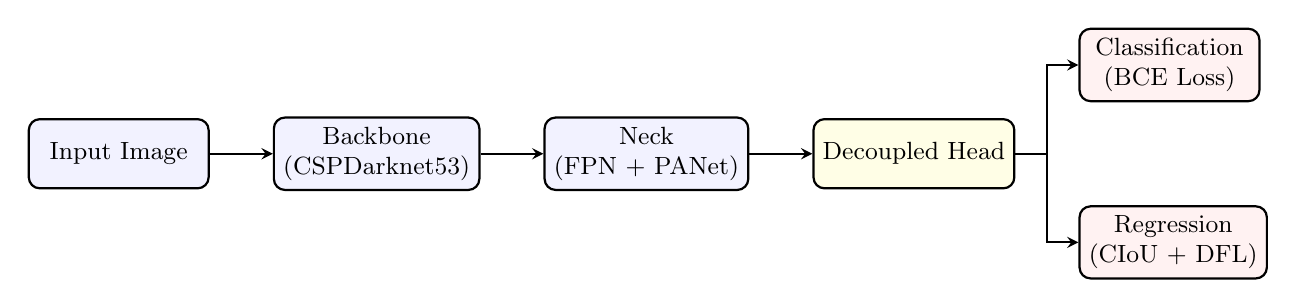
\begin{tikzpicture}[>=stealth, thick]
    \tikzset{
        block/.style={draw, fill=blue!5, rectangle, minimum height=2.5em, minimum width=6.5em, rounded corners, align=center, font=\small},
        split/.style={draw, fill=yellow!10, rectangle, minimum height=2.5em, minimum width=6.5em, rounded corners, align=center, font=\small},
        head/.style={draw, fill=red!5, rectangle, minimum height=2.5em, minimum width=6.5em, rounded corners, align=center, font=\small},
        line/.style={draw, ->, >=stealth, thick}
    }
    \node [block] (input) {Input Image};
    \node [block, right=0.8cm of input] (backbone) {Backbone\\(CSPDarknet53)};
    \node [block, right=0.8cm of backbone] (neck) {Neck\\(FPN + PANet)};
    \node [split, right=0.8cm of neck] (decoupled) {Decoupled Head};
    \node [head, above right=0.2cm and 0.8cm of decoupled] (cls) {Classification\\(BCE Loss)};
    \node [head, below right=0.2cm and 0.8cm of decoupled] (reg) {Regression\\(CIoU + DFL)};
    
    \path [line] (input) -- (backbone);
    \path [line] (backbone) -- (neck);
    \path [line] (neck) -- (decoupled);
    \draw [line] (decoupled.east) -- +(0.4,0) |- (cls.west);
    \draw [line] (decoupled.east) -- +(0.4,0) |- (reg.west);
\end{tikzpicture}
\caption{YOLOv8 Single-Stage Object Detection Pipeline Architecture~\cite{yolov8}.}
\label{fig:yolov8_arch}
\end{figure}

The anchor-free regression directly predicts the distances from the candidate point to the four boundaries of the bounding box. The model optimizes a joint loss function:
\begin{equation}
    \mathcal{L}_{\text{total}} = \lambda_1 \mathcal{L}_{\text{BCE}} + \lambda_2 \mathcal{L}_{\text{CIoU}} + \lambda_3 \mathcal{L}_{\text{DFL}}
\end{equation}
where $\mathcal{L}_{\text{BCE}}$ is the Binary Cross Entropy loss for classification. The Complete Intersection over Union ($\mathcal{L}_{\text{CIoU}}$) measures bounding box overlap, center distance, and aspect ratio consistency:
\begin{equation}
    \mathcal{L}_{\text{CIoU}} = 1 - \text{IoU} + \frac{\rho^2(\mathbf{b}, \mathbf{b}^{\text{gt}})}{c^2} + \alpha v
\end{equation}
where $\rho(\cdot)$ represents Euclidean distance between the predicted box $\mathbf{b}$ and ground-truth box $\mathbf{b}^{\text{gt}}$ center points, $c$ is the diagonal length of the smallest enclosing box, $v = \frac{4}{\pi^2} (\arctan \frac{w^{\text{gt}}}{h^{\text{gt}}} - \arctan \frac{w}{h})^2$ and $\alpha = \frac{v}{(1-\text{IoU})+v}$ is a weight parameter. The Distribution Focal Loss ($\mathcal{L}_{\text{DFL}}$) focuses the network on the distributions of boundary coordinates to handle boundary uncertainty:
\begin{equation}
    \mathcal{L}_{\text{DFL}}(P_i, P_{i+1}) = - \left( (y_{i+1} - y) \log(P_i) + (y - y_i) \log(P_{i+1}) \right)
\end{equation}
where $y$ is the ground-truth coordinate, $y_i, y_{i+1}$ are the integer boundary bins surrounding $y$, and $P_i, P_{i+1}$ are the predicted probabilities. This architecture minimizes latency and is highly optimized for edge deployment. In this thesis, we replace the multiple parallel detectors of the original Pylot setup with a single trained YOLOv8 model to establish a streamlined, real-time perception pipeline.

\section{Dynamic State Estimation and Motion Modules}
\label{sec:estimation_motion}

Following the perception step, several downstream modules process obstacle state representations to determine vehicle control commands.

\subsection{Obstacle Tracking (SORT)}
Object detection only runs on individual frames; it does not associate detections across time. As defined by Gog et al.~\cite{erdos_pylot}, the tracking component estimates the bounding boxes of objects over time, and maintains consistent identifiers for the objects across detections. It utilizes bounding boxes from the \texttt{ObstacleMessage} and communicates results via an \texttt{ObstacleTrajectoryMessage}. Pylot provides multiple trackers, and in this thesis, we utilize the Simple Online and Realtime Tracking (SORT) algorithm~\cite{sort_tracker}. 
\begin{itemize}
    \item \textbf{Role}: To associate obstacle detections across sequential frames, maintain persistent obstacle IDs, and estimate their dynamic states (position and velocity).
    \item \textbf{Inputs}: 3D bounding boxes of obstacles, class labels, and detection confidence scores from the perception module.
    \item \textbf{Outputs}: Tracked obstacle states, containing unique tracking IDs, persistent 3D bounding boxes, and estimated velocity vectors.
\end{itemize}
The flow diagram of SORT is illustrated in Figure~\ref{fig:sort_flow}.

\begin{figure}[H]
\centering
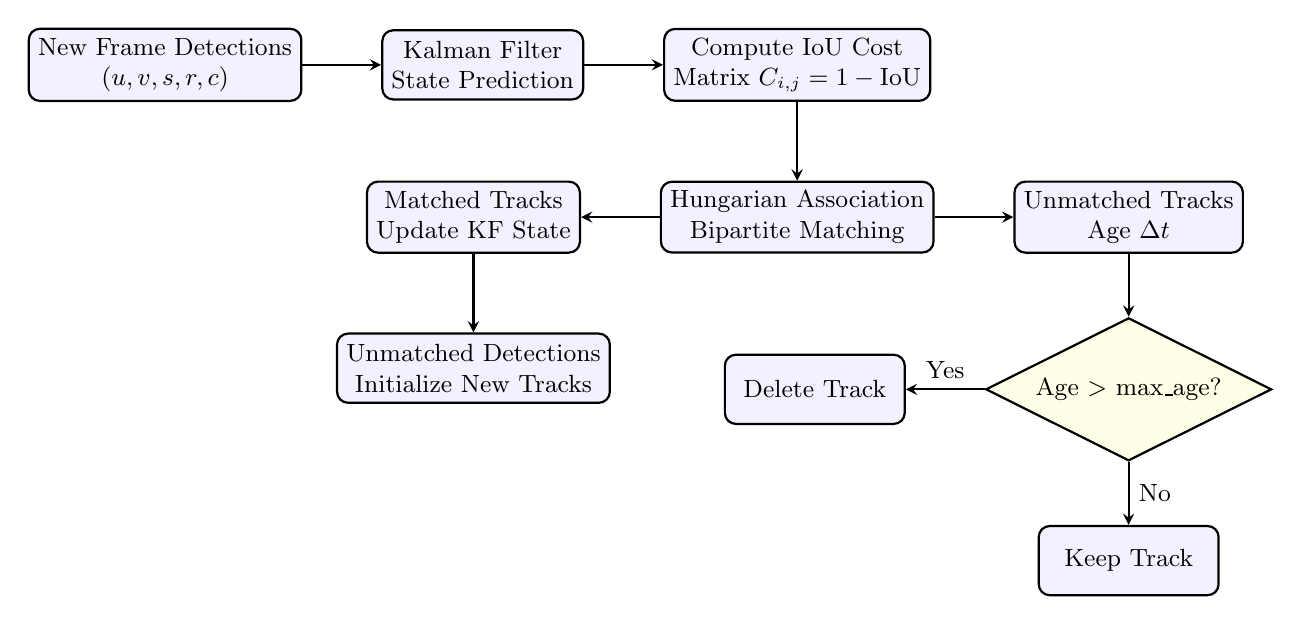
\begin{tikzpicture}[>=stealth, thick]
    \tikzset{
        processstep/.style={draw, fill=blue!5, rectangle, minimum height=2.5em, minimum width=6.5em, rounded corners, align=center, font=\small},
        decision/.style={draw, fill=yellow!10, diamond, aspect=2, minimum width=6.5em, align=center, font=\small},
        line/.style={draw, ->, >=stealth, thick}
    }
    \node [processstep] (det) {New Frame Detections\\$(u, v, s, r, c)$};
    \node [processstep, right=1.0cm of det] (predict) {Kalman Filter\\State Prediction};
    \node [processstep, right=1.0cm of predict] (cost) {Compute IoU Cost\\Matrix $C_{i,j} = 1 - \text{IoU}$};
    \node [processstep, below=1cm of cost] (hungarian) {Hungarian Association\\Bipartite Matching};
    
    \node [processstep, left=1.0cm of hungarian] (matched) {Matched Tracks\\Update KF State};
    \node [processstep, below=1cm of matched] (unmatched_det) {Unmatched Detections\\Initialize New Tracks};
    \node [processstep, right=1.0cm of hungarian] (unmatched_track) {Unmatched Tracks\\Age $\Delta t$};
    \node [decision, below=0.8cm of unmatched_track] (age_check) {Age $>$ max\_age?};
    \node [processstep, left=1cm of age_check] (delete) {Delete Track};
    \node [processstep, below=0.8cm of age_check] (keep) {Keep Track};

    \path [line] (det) -- (predict);
    \path [line] (predict) -- (cost);
    \path [line] (cost) -- (hungarian);
    \path [line] (hungarian) -- (matched);
    \path [line] (hungarian) -- (unmatched_track);
    \path [line] (matched) -- (unmatched_det);
    \path [line] (unmatched_track) -- (age_check);
    
    \draw [line] (age_check.west) -- node[above, font=\small] {Yes} (delete.east);
    \draw [line] (age_check.south) -- node[right, font=\small] {No} (keep.north);
\end{tikzpicture}
\caption{SORT Obstacle Tracking Workflow~\cite{sort_tracker}.}
\label{fig:sort_flow}
\end{figure}

SORT models the state of each tracking target using a 7-dimensional vector:
\begin{equation}
    \mathbf{x} = [u, v, s, r, \dot{u}, \dot{v}, \dot{s}]^{\text{T}}
\end{equation}
where $(u, v)$ is the 2D pixel center of the bounding box, $s$ is the scale (area of the box), $r$ is the aspect ratio (width over height, assumed constant), and $\dot{u}, \dot{v}, \dot{s}$ are their respective velocities. 
A linear constant velocity model is used to predict the target's state in the next frame:
\begin{equation}
    \mathbf{x}_{k} = \mathbf{F} \mathbf{x}_{k-1} + \mathbf{w}_k, \quad \mathbf{z}_k = \mathbf{H} \mathbf{x}_k + \mathbf{v}_k
\end{equation}
where $\mathbf{F}$ is the $7 \times 7$ state transition matrix, mapping the previous state to the current state based on physical kinematics. Assuming a constant frame rate $\Delta t = 1$, the transition matrix is defined as:
\begin{equation}
    \mathbf{F} = \begin{bmatrix}
    1 & 0 & 0 & 0 & 1 & 0 & 0 \\
    0 & 1 & 0 & 0 & 0 & 1 & 0 \\
    0 & 0 & 1 & 0 & 0 & 0 & 1 \\
    0 & 0 & 0 & 1 & 0 & 0 & 0 \\
    0 & 0 & 0 & 0 & 1 & 0 & 0 \\
    0 & 0 & 0 & 0 & 0 & 1 & 0 \\
    0 & 0 & 0 & 0 & 0 & 0 & 1
    \end{bmatrix}
\end{equation}
The matrix $\mathbf{H}$ is the $4 \times 7$ measurement matrix that projects the 7D state space into the 4D measurement space (since the detector only observes position and scale, not velocity):
\begin{equation}
    \mathbf{H} = \begin{bmatrix}
    1 & 0 & 0 & 0 & 0 & 0 & 0 \\
    0 & 1 & 0 & 0 & 0 & 0 & 0 \\
    0 & 0 & 1 & 0 & 0 & 0 & 0 \\
    0 & 0 & 0 & 1 & 0 & 0 & 0
    \end{bmatrix}
\end{equation}
The variables $\mathbf{w}_k \sim \mathcal{N}(0, \mathbf{Q})$ and $\mathbf{v}_k \sim \mathcal{N}(0, \mathbf{R})$ represent the process noise and measurement noise covariances, respectively. At every timestamp, the Kalman filter executes a two-step recursive process:
\begin{enumerate}
    \item \textbf{Predict:} Estimate the \textit{a priori} state and error covariance matrix $\mathbf{P}$:
    \begin{align}
        \hat{\mathbf{x}}_{k|k-1} &= \mathbf{F} \hat{\mathbf{x}}_{k-1|k-1} \\
        \mathbf{P}_{k|k-1} &= \mathbf{F} \mathbf{P}_{k-1|k-1} \mathbf{F}^{\text{T}} + \mathbf{Q}
    \end{align}
    \item \textbf{Update:} Incorporate the new bounding box measurement $\mathbf{z}_k$ by calculating the Kalman Gain $\mathbf{K}_k$, and computing the \textit{a posteriori} state estimate:
    \begin{align}
        \mathbf{K}_k &= \mathbf{P}_{k|k-1} \mathbf{H}^{\text{T}} (\mathbf{H} \mathbf{P}_{k|k-1} \mathbf{H}^{\text{T}} + \mathbf{R})^{-1} \\
        \hat{\mathbf{x}}_{k|k} &= \hat{\mathbf{x}}_{k|k-1} + \mathbf{K}_k (\mathbf{z}_k - \mathbf{H} \hat{\mathbf{x}}_{k|k-1}) \\
        \mathbf{P}_{k|k} &= (\mathbf{I} - \mathbf{K}_k \mathbf{H}) \mathbf{P}_{k|k-1}
    \end{align}
\end{enumerate}
This highly optimized linear algebraic process requires sub-millisecond execution times, making it uniquely suited for the stringent latency constraints of modular autonomous driving platforms like Pylot.

To associate detections with existing tracks, an assignment cost matrix is constructed using the Intersection over Union (IoU) distance:
\begin{equation}
    C_{i,j} = 1 - \text{IoU}(\text{Target}_i, \text{Detection}_j)
\end{equation}
The Hungarian algorithm is applied to find the optimal bipartite matching. Detections with matching overlap below $\text{IoU}_{\text{min}}$ (e.g. 0.3) are rejected. Unmatched detections initialize new tracks with zero velocity, and tracks that remain unmatched for more than $\text{max\_age}$ frames are deleted.

\subsection{Obstacle Prediction}
To plan safe paths, the vehicle must predict the future movements of surrounding obstacles. As detailed in the Pylot platform~\cite{erdos_pylot}, the prediction module uses the tracked history of nearby agents, along with scene context, to predict future agent behavior. Specifically, it receives the bounding box and the identifier of each obstacle at every time instant through the \texttt{ObstacleTrajectoryMessage}, and generates an \texttt{ObstaclePredictionMessage} containing the past and the predicted trajectory for each obstacle. For this pipeline, the prediction module subscribes to the tracked object streams and fits a linear extrapolation model. 
\begin{itemize}
    \item \textbf{Role}: To forecast the future spatial positions of surrounding dynamic obstacles over a specified future time horizon.
    \item \textbf{Inputs}: Tracked obstacles with unique IDs, current positions, and historical trajectory coordinates from the tracking module.
    \item \textbf{Outputs}: Predicted future trajectories, represented as a sequence of future 3D coordinates for each tracked obstacle.
\end{itemize}
Figure~\ref{fig:linear_prediction} illustrates this least-squares linear prediction process.

\begin{figure}[H]
\centering
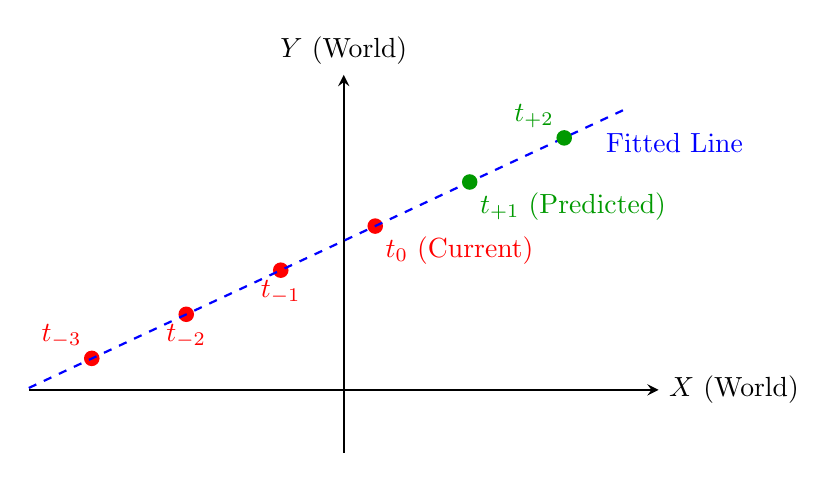
\begin{tikzpicture}[>=stealth, scale=0.8, thick]
    % Draw grid / axes
    \draw[->] (-5,0) -- (5,0) node[right] {$X$ (World)};
    \draw[->] (0,-1) -- (0,5) node[above] {$Y$ (World)};
    
    % Draw historical points (crosses/dots)
    \filldraw[red] (-4, 0.5) circle (3pt) node[above left] {$t_{-3}$};
    \filldraw[red] (-2.5, 1.2) circle (3pt) node[below] {$t_{-2}$};
    \filldraw[red] (-1.0, 1.9) circle (3pt) node[below] {$t_{-1}$};
    \filldraw[red] (0.5, 2.6) circle (3pt) node[below right] {$t_{0}$ (Current)};
    
    % Draw regression line
    \draw[blue, thick, dashed] (-5, 0.03) -- (4.5, 4.47);
    \node[blue, below right] at (4.0, 4.23) {Fitted Line};
    
    % Draw future prediction points
    \filldraw[green!60!black] (2.0, 3.3) circle (3pt) node[below right] {$t_{+1}$ (Predicted)};
    \filldraw[green!60!black] (3.5, 4.0) circle (3pt) node[above left] {$t_{+2}$};
\end{tikzpicture}
\caption{Linear Trajectory Prediction Fitting and Extrapolation~\cite{erdos_pylot}.}
\label{fig:linear_prediction}
\end{figure}

The module calculates the current velocity and heading of each obstacle based on historical tracking states. Given $N$ past location coordinates $(x_t, y_t)$ for $t = 0, -1, \dots, -(N-1)$ from SORT, it models $x(t) = w_{x,1} t + w_{x,0}$ and $y(t) = w_{y,1} t + w_{y,0}$. The parameter matrix $\mathbf{W}$ is computed via least-squares:
\begin{equation}
    \mathbf{W} = (\mathbf{T}^{\text{T}} \mathbf{T})^{-1} \mathbf{T}^{\text{T}} \mathbf{XY}
\end{equation}
where $\mathbf{XY} \in \mathbb{R}^{N \times 2}$ is the coordinate matrix and $\mathbf{T} \in \mathbb{R}^{N \times 2}$ is the time step matrix:
\begin{equation}
    \mathbf{T} = \begin{pmatrix} 0 & 1 \\ -1 & 1 \\ \vdots & \vdots \\ -(N-1) & 1 \end{pmatrix}, \quad \mathbf{W} = \begin{pmatrix} w_{x,1} & w_{y,1} \\ w_{x,0} & w_{y,0} \end{pmatrix}
\end{equation}
Future positions for the prediction horizon $H$ (at times $t = 1, 2, \dots, H$) are projected:
\begin{equation}
    \mathbf{XY}_{\text{future}} = \mathbf{T}_{\text{future}} \mathbf{W}
\end{equation}
where $\mathbf{T}_{\text{future}} \in \mathbb{R}^{H \times 2}$ has rows $(j, 1)$ for $j = 1, \dots, H$.

\subsection{Waypoint Planning}
According to the Pylot methodology~\cite{erdos_pylot}, the goal of the planning module is to produce a safe, comfortable, and feasible trajectory that accounts for the present and future possible states of the environment. To achieve this, the planning module synchronizes the output from all other modules to construct a \texttt{World} representation containing past and future trajectories of all agents, alongside static objects like traffic lights and signs. The module comprises route, behavioral, and motion planners. The waypoint planner receives the vehicle's localization pose, the target destination, traffic light states, and predicted obstacle trajectories. It plans a set of waypoints (coordinates) and target speeds. Pylot implements three core planning algorithms:
\begin{itemize}
    \item \textbf{Role}: To compute a safe, kinematically-feasible, and collision-free path of waypoints and target velocities leading to the destination.
    \item \textbf{Inputs}: Current ego-vehicle localization pose, target destination route/waypoints, traffic light states, and predicted future trajectories of dynamic obstacles.
    \item \textbf{Outputs}: A sequence of target waypoints (world coordinates) and target velocities for each waypoint.
\end{itemize}

\subsubsection{Frenet Optimal Trajectory}
The Frenet Optimal Trajectory planner~\cite{frenet_planner} evaluates candidate trajectories in a coordinate frame aligned with the road centerline (Frenet frame), as shown in Figure~\ref{fig:frenet_frame}.

\begin{figure}[H]
\centering
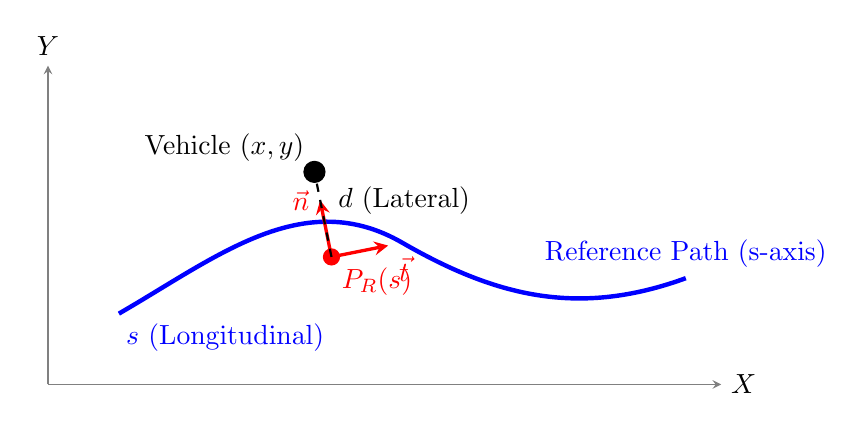
\begin{tikzpicture}[>=stealth, scale=0.9, thick]
    % Cartesian axes
    \draw[->, gray, thin] (-1,-1) -- (8.5,-1) node[right, black] {$X$};
    \draw[->, gray, thin] (-1,-1) -- (-1,3.5) node[above, black] {$Y$};
    
    % Reference centerline curve
    \draw[blue, ultra thick] (0,0) to[out=30, in=150] (4,1) to[out=-30, in=200] (8,0.5);
    \node[blue, above] at (8,0.5) {Reference Path (s-axis)};
    
    % Vehicle position
    \filldraw[black] (2.76, 2.0) circle (4pt) node[above left] {Vehicle $(x, y)$};
    
    % Projection point on reference path
    \filldraw[red] (3.0, 0.8) circle (3pt) node[below right] {$P_R(s)$};
    
    % Tangent and Normal vectors at PR
    \draw[->, red, very thick] (3.0, 0.8) -- (3.8, 0.96) node[below right] {$\vec{t}$};
    \draw[->, red, very thick] (3.0, 0.8) -- (2.84, 1.6) node[left] {$\vec{n}$};
    
    % Projection line representing d
    \draw[dashed, black] (3.0, 0.8) -- (2.76, 2.0);
    \node[right] at (2.95, 1.6) {$d$ (Lateral)};
    
    % Longitudinal coordinate s
    \node[blue, below] at (1.5, 0.0) {$s$ (Longitudinal)};
\end{tikzpicture}
\caption{Frenet Frame Coordinate System representing longitudinal distance $s$ and lateral displacement $d$~\cite{frenet_planner}.}
\label{fig:frenet_frame}
\end{figure}

The position is represented by $s(t)$ (longitudinal displacement along the centerline) and $d(t)$ (lateral displacement perpendicular to it). Lateral trajectories are generated as a quintic polynomial to allow matching boundary conditions of position, velocity, and acceleration:
\begin{equation}
    d(t) = a_0 + a_1 t + a_2 t^2 + a_3 t^3 + a_4 t^4 + a_5 t^5
\end{equation}
Longitudinal trajectories are modeled as a quartic polynomial for velocity keeping:
\begin{equation}
    s(t) = b_0 + b_1 t + b_2 t^2 + b_3 t^3 + b_4 t^4
\end{equation}
The planner minimizes cost functions evaluating jerk (comfort), time, lateral offset, and target speed deviation:
\begin{align}
    C_{\text{lat}} &= k_j \int \dddot{d}(t)^2 dt + k_t t_f^2 + k_d d(t_f)^2 \\
    C_{\text{lon}} &= k_j \int \dddot{s}(t)^2 dt + k_t t_f^2 + k_s (\dot{s}(t_f) - v_{\text{target}})^2
\end{align}
Total cost $C_{\text{total}} = k_{\text{lat}} C_{\text{lat}} + k_{\text{lon}} C_{\text{lon}}$ is evaluated, and the minimum-cost trajectory that satisfies kinodynamic constraints (maximum curvature, acceleration, speed) and avoids predicted obstacle polygons is chosen.

\subsubsection{RRT* (Rapidly-exploring Random Trees)}
RRT*~\cite{rrt_star} is an incremental, sampling-based path planner that builds a tree $\mathcal{T} = (\mathcal{V}, \mathcal{E})$ of valid trajectories through the configuration space. 
In each iteration, the planner:
\begin{enumerate}
    \item Samples a random obstacle-free coordinate $\mathbf{x}_{\text{rand}} \in X_{\text{free}}$.
    \item Finds the closest node $\mathbf{x}_{\text{nearest}} \in \mathcal{V}$.
    \item Steers a distance $\eta$ from $\mathbf{x}_{\text{nearest}}$ toward $\mathbf{x}_{\text{rand}}$ to generate a new node candidate $\mathbf{x}_{\text{new}}$.
    \item If the path between $\mathbf{x}_{\text{nearest}}$ and $\mathbf{x}_{\text{new}}$ is collision-free, it selects the parent $\mathbf{x}_{\text{parent}} \in \mathcal{V} \cap \text{Ball}(\mathbf{x}_{\text{new}}, r)$ that minimizes the path cost from the root to $\mathbf{x}_{\text{new}}$.
    \item Rewires the tree: for each neighboring node $\mathbf{x}_{\text{near}} \in \mathcal{V} \cap \text{Ball}(\mathbf{x}_{\text{new}}, r)$, if reaching $\mathbf{x}_{\text{near}}$ via $\mathbf{x}_{\text{new}}$ results in a lower path cost than its current parent, the parent pointer of $\mathbf{x}_{\text{near}}$ is updated to $\mathbf{x}_{\text{new}}$.
\end{enumerate}
This rewiring property guarantees asymptotic optimality, converging toward the shortest collision-free path.

\subsubsection{Hybrid A*}
Hybrid A*~\cite{hybrid_a_star} is a search-based planner that extends the traditional $A^*$ grid search to continuous vehicle configuration states $(x, y, \theta)$ to ensure kinematically feasible trajectories. 
While standard $A^*$ searches discrete grid nodes, leading to sharp turns that a vehicle cannot execute, Hybrid A* associates each search node with a continuous state. The continuous node transitions are computed using the kinematic bicycle model:
\begin{equation}
    \dot{x} = v \cos\theta, \quad \dot{y} = v \sin\theta, \quad \dot{\theta} = \frac{v}{L} \tan\delta
\end{equation}
where $v$ is the velocity, $\theta$ is the heading yaw, $\delta \in [\delta_{\text{min}}, \delta_{\text{max}}]$ is the steering angle, and $L$ is the vehicle wheelbase. Node pruning is performed by partitioning the search space into discrete 3D grid bins $(x_d, y_d, \theta_d)$, keeping only the lowest-cost continuous node per bin. It guides the search using two heuristics: the non-holonomic-without-obstacles heuristic (Reed-Shepp curves) and the obstacle-aware-2D heuristic.

\subsection{Vehicle Control (PID)}
As described in the Pylot architecture~\cite{erdos_pylot}, the control module receives waypoints and target speeds from the planning module. It aims to closely follow the provided waypoints while maintaining its target speed. The control module translates planned waypoints and target velocities into physical actuation commands: steering angle, throttle, and brake, and sends these to the simulator. Pylot employs Proportional-Integral-Derivative (PID) controllers~\cite{pid_control}, whose feedback loop is shown in Figure~\ref{fig:pid_loop}.
\begin{itemize}
    \item \textbf{Role}: To generate low-level physical actuation commands that steer, accelerate, and decelerate the vehicle to follow the planned waypoints.
    \item \textbf{Inputs}: Planned target waypoints, target speeds from the planning module, and the current state of the vehicle (position, orientation, current velocity).
    \item \textbf{Outputs}: Actuation commands sent to the simulator/actuators (throttle percentage, braking pressure, steering angle).
\end{itemize}

\begin{figure}[H]
\centering
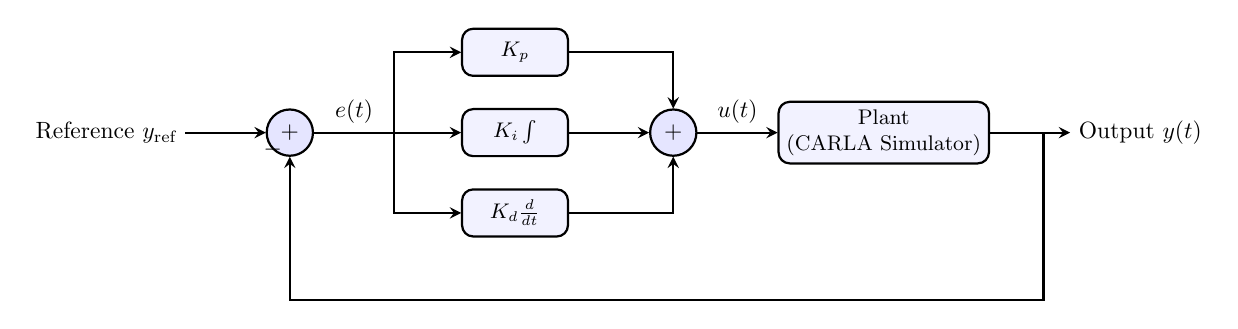
\begin{tikzpicture}[>=stealth, thick, scale=0.85, transform shape]
    \tikzset{
        block/.style={draw, fill=blue!5, rectangle, minimum height=2em, minimum width=4.5em, rounded corners, align=center, font=\small},
        sum/.style={draw, fill=blue!10, circle, minimum size=1.5em},
        line/.style={draw, ->, >=stealth, thick}
    }
    \node (ref) {Reference $y_{\text{ref}}$};
    \node [sum, right=1.2cm of ref] (sum) {$+$};
    \node [block, right=2.2cm of sum, yshift=1.2cm] (p) {$K_p$};
    \node [block, right=2.2cm of sum] (i) {$K_i \int$};
    \node [block, right=2.2cm of sum, yshift=-1.2cm] (d) {$K_d \frac{d}{dt}$};
    \node [sum, right=1.2cm of i] (sum2) {$+$};
    \node [block, right=1.2cm of sum2] (plant) {Plant\\(CARLA Simulator)};
    \node [right=1.2cm of plant] (out) {Output $y(t)$};
    
    \path [line] (ref) -- (sum);
    \coordinate (branch1) at ($(sum.east) + (1.2, 0)$);
    \draw [thick] (sum.east) -- node[above] {$e(t)$} (branch1);
    \path [line] (branch1) |- (p.west);
    \path [line] (branch1) -- (i.west);
    \path [line] (branch1) |- (d.west);
    
    \path [line] (p.east) -| (sum2);
    \path [line] (i.east) -- (sum2);
    \path [line] (d.east) -| (sum2);
    
    \path [line] (sum2) -- node[above] {$u(t)$} (plant);
    \path [line] (plant) -- (out);
    
    % Feedback loop
    \draw [line] (plant.east) -- +(0.8,0) |- +(0,-2.5) -| (sum.south);
    \node at (sum.south west) {$-$};
\end{tikzpicture}
\caption{Proportional-Integral-Derivative (PID) Controller Feedback Loop~\cite{pid_control}.}
\label{fig:pid_loop}
\end{figure}

The controllers track target values using the error $e(t) = y_{\text{ref}}(t) - y(t)$:
\begin{equation}
    u(t) = K_p e(t) + K_i \int_0^t e(\tau) d\tau + K_d \frac{de(t)}{dt}
\end{equation}

\subsubsection{Lateral PID Controller}
The lateral controller minimizes the steering error by adjusting the steering wheel angle. Let $\mathbf{h} = [\cos\psi, \sin\psi]^{\text{T}}$ be the current heading vector of the vehicle, and $\mathbf{w} = [x_{\text{wp}} - x_{\text{veh}}, y_{\text{wp}} - y_{\text{veh}}]^{\text{T}}$ be the vector pointing from the vehicle to the closest target waypoint. The heading error angle $\theta_e$ is computed as:
\begin{equation}
    \theta_e = \text{sgn}(\mathbf{h} \times \mathbf{w}) \arccos \left( \frac{\mathbf{h} \cdot \mathbf{w}}{\|\mathbf{h}\| \|\mathbf{w}\|} \right)
\end{equation}
where $\text{sgn}(\mathbf{h} \times \mathbf{w}) = \text{sign}(h_x w_y - h_y w_x)$ determines whether the vehicle needs to turn left or right. The steering command is:
\begin{equation}
    u_{\text{steer}}(t) = K_{p,\theta} \theta_e(t) + K_{i,\theta} \int_0^t \theta_e(\tau) d\tau + K_{d,\theta} \frac{d\theta_e(t)}{dt}
\end{equation}
which is clipped between $-1.0$ (hard left) and $1.0$ (hard right).

\subsubsection{Longitudinal PID Controller}
The longitudinal controller tracks the target velocity by comparing the vehicle's current speed $v(t)$ with the target speed $v_{\text{target}}(t)$:
\begin{equation}
    e_v(t) = (v_{\text{target}}(t) - v(t)) \cdot 3.6
\end{equation}
The error is scaled to km/h. The actuation command $u_{\text{accel}}(t)$ is:
\begin{equation}
    u_{\text{accel}}(t) = K_{p,v} e_v(t) + K_{i,v} \int_0^t e_v(\tau) d\tau + K_{d,v} \frac{de_v(t)}{dt}
\end{equation}
The output $u_{\text{accel}}(t) \in [-1.0, 1.0]$ is clipped. A positive value is mapped to throttle (gas pedal), and a negative value is mapped to braking pressure.

\subsection{Model Predictive Control (MPC)}
While PID controllers are highly reactive and computationally inexpensive, they only account for instantaneous errors and are fundamentally ignorant of the vehicle's physical limits and future trajectory curves. This can lead to dangerous oversteering or oscillation at high velocities. To mitigate this, advanced iterations of the Pylot stack utilize Model Predictive Control (MPC).

MPC formulates the path tracking task as a constrained, receding horizon optimization problem. Instead of blindly reacting to the current error, MPC utilizes a mathematical model of the vehicle's kinematics to simulate and evaluate various actuation commands over a future time horizon of length $N$. 

Let the state vector of the vehicle be $\mathbf{z} = [x, y, v, \theta]^{\text{T}}$ and the control input vector be $\mathbf{u} = [a, \delta]^{\text{T}}$, where $a$ is longitudinal acceleration and $\delta$ is the steering angle. The discrete-time kinematic bicycle model updates the state as follows:
\begin{align}
    x_{k+1} &= x_k + v_k \cos(\theta_k) \Delta t \\
    y_{k+1} &= y_k + v_k \sin(\theta_k) \Delta t \\
    v_{k+1} &= v_k + a_k \Delta t \\
    \theta_{k+1} &= \theta_k + \frac{v_k}{L} \tan(\delta_k) \Delta t
\end{align}
where $L$ is the vehicle wheelbase. At each control step, MPC minimizes a multi-objective cost function $J$:
\begin{equation}
    \min_{\mathbf{u}_0, \dots, \mathbf{u}_{N-1}} J = \sum_{k=1}^{N} \left( \|\mathbf{z}_k - \mathbf{z}_{k,\text{ref}}\|_{\mathbf{Q}}^2 + \|\mathbf{u}_k\|_{\mathbf{R}}^2 + \|\Delta \mathbf{u}_k\|_{\mathbf{S}}^2 \right)
\end{equation}
where $\mathbf{z}_{k,\text{ref}}$ is the target waypoint state from the planner, $\Delta \mathbf{u}_k$ is the rate of change of the control inputs (representing passenger comfort/jerk), and $\mathbf{Q}, \mathbf{R}, \mathbf{S}$ are positive-definite weighting matrices. 

Crucially, this optimization is subject to strict physical and safety constraints:
\begin{align}
    \mathbf{z}_{\text{min}} \le \mathbf{z}_k \le \mathbf{z}_{\text{max}} \quad &\text{(State boundaries, e.g., max speed)} \\
    \mathbf{u}_{\text{min}} \le \mathbf{u}_k \le \mathbf{u}_{\text{max}} \quad &\text{(Actuation limits, e.g., max steering angle $\pm 30^{\circ}$)} \\
    |\Delta \mathbf{u}_k| \le \Delta \mathbf{u}_{\text{max}} \quad &\text{(Actuation rate limits, e.g., steering wheel motor speed)}
\end{align}

Because solving this non-linear optimization program (NLP) over a time horizon requires significant computational resources, the latency of the MPC solver must be explicitly accounted for in the Pylot dataflow graph. If the solver latency exceeds the simulation tick duration, the vehicle will execute stale commands, potentially violating the very safety boundaries the MPC was designed to uphold.

\section{Latency-Accuracy Tradeoffs and Timely Accuracy}
\label{sec:timely_accuracy}
A primary motivation for utilizing the Pylot platform is to evaluate the latency-accuracy tradeoff of the modular pipeline. Traditional offline metrics such as mean Average Precision (mAP) or Intersection over Union (IoU) evaluate a model's output against the ground truth at the exact moment the sensor data was captured. However, in an autonomous driving context, the environment continues to evolve while the perception model is executing. 

To address this, Pylot introduces the concept of \textbf{Timely Accuracy}~\cite{erdos_pylot}. Timely accuracy evaluates a module's output against the ground truth at the moment the computation \textit{finishes}. If an object detector takes a computational time of $l_t$ to process an image captured at time $t_1$, the output bounding boxes are evaluated against the true position of objects at time $t_2 = t_1 + l_t$.

The timely accuracy fundamentally depends on both the algorithmic runtime and the ego-vehicle's velocity. Empirical studies using Pylot have demonstrated that as vehicle speed increases, the timely accuracy of slow, high-precision models (like Faster R-CNN) degrades exponentially faster than that of fast, lower-precision models (like SSD or YOLOv8). At 10 m/s, a heavy model may achieve higher timely accuracy, but at 40 m/s, the fast model decisively outperforms it because the heavy model's output is obsolete by the time it is produced. This paradigm shift proves that real-time autonomous driving stacks must be meticulously optimized for inference latency, not just theoretical offline accuracy.



\chapter{Methodology and Modular Integration}

This chapter details the dataflow graph structure of the integrated Pylot pipeline, the process of replacing Pylot's original multi-model perception with a streamlined single YOLOv8 model, and how these components are wired to achieve closed-loop autonomous driving.

\section{The Pylot Dataflow Graph}
\label{sec:dataflow_graph}
The autonomous driving stack is constructed as a directed acyclic graph (DAG) of ERDOS operators. Figure~\ref{fig:pylot_diagram} illustrates the dataflow path of our system:

\begin{figure}[htbp]
    \centering
    \resizebox{\textwidth}{!}{%
    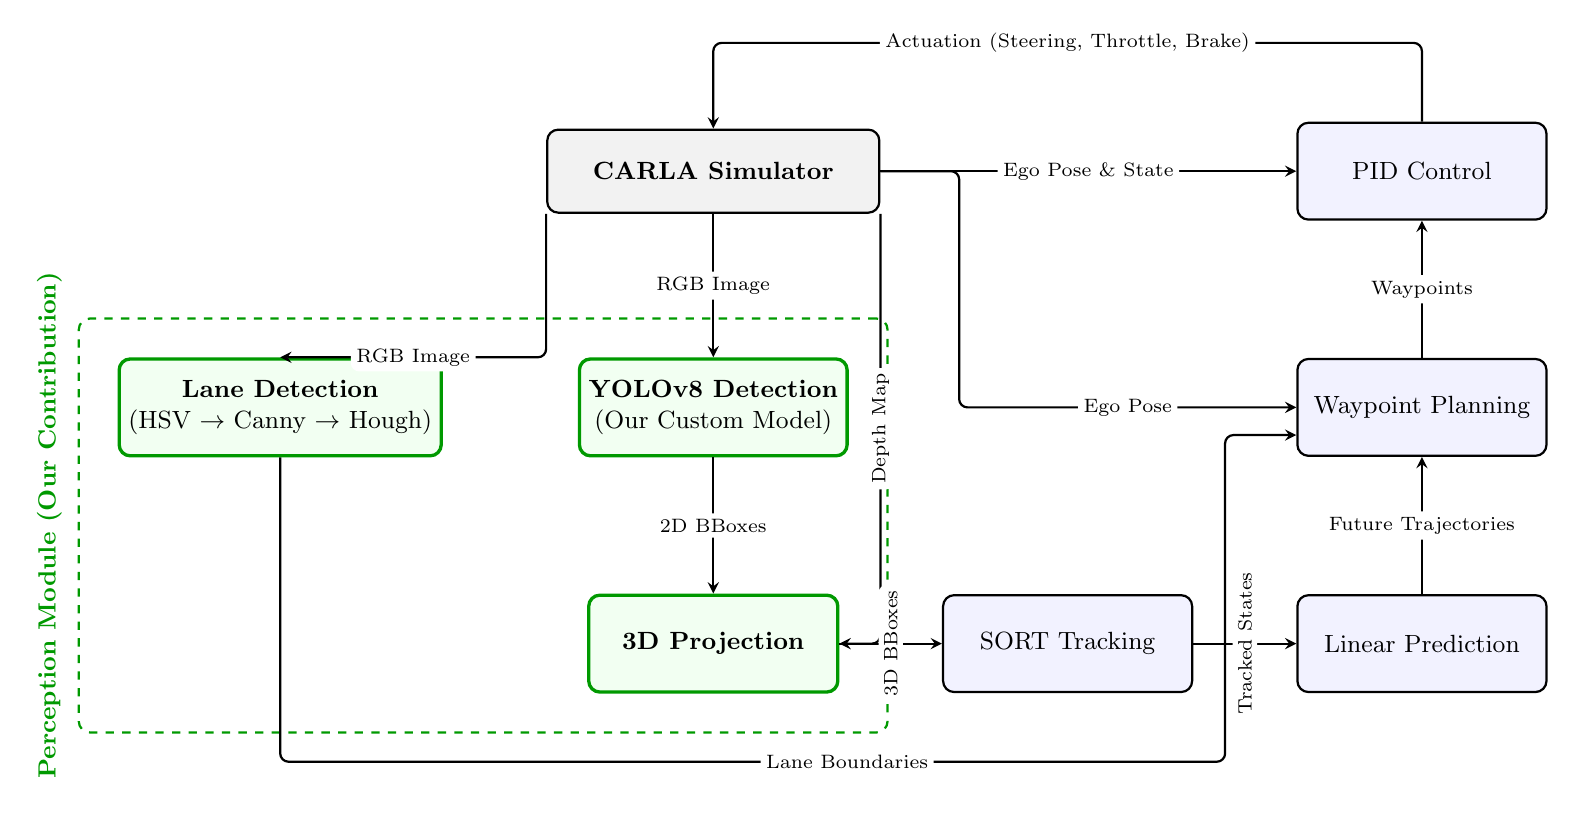
\begin{tikzpicture}[>=stealth, thick]
        \tikzset{
            sensor/.style={draw, fill=gray!10, rectangle, minimum height=3em, minimum width=12em, rounded corners, align=center, font=\small\bfseries},
            module/.style={draw, fill=blue!5, rectangle, minimum height=3.5em, minimum width=9em, rounded corners, align=center, font=\small},
            highlight/.style={draw=green!60!black, fill=green!5, rectangle, minimum height=3.5em, minimum width=9em, rounded corners, align=center, font=\small, line width=1.2pt},
            io/.style={font=\scriptsize, align=center, fill=white, inner sep=2pt},
            line/.style={draw, ->, >=stealth, thick, rounded corners=3pt}
        }
        
        % Simulator
        \node [sensor] (carla) at (2, 0) {CARLA Simulator};
        
        % Perception Module
        \node [highlight] (lane) at (-3.5, -3) {\textbf{Lane Detection}\\(HSV $\rightarrow$ Canny $\rightarrow$ Hough)};
        \node [highlight] (yolo) at (2, -3) {\textbf{YOLOv8 Detection}\\(Our Custom Model)};
        \node [highlight] (proj) at (2, -6) {\textbf{3D Projection}};
        
        % Grouping Perception
        \node[draw=green!60!black, dashed, rounded corners, fit=(lane) (yolo) (proj), inner sep=14pt] (perception_box) {};
        \node[green!60!black, font=\small\bfseries, rotate=90, anchor=south, yshift=2pt] at (perception_box.west) {Perception Module (Our Contribution)};
        
        % Downstream Modules
        \node [module] (sort) at (6.5, -6) {SORT Tracking};
        \node [module] (pred) at (11, -6) {Linear Prediction};
        \node [module] (plan) at (11, -3) {Waypoint Planning};
        \node [module] (control) at (11, 0) {PID Control};
        
        % Connections from CARLA
        \draw [line] (carla.south) -- node[io] {RGB Image} (yolo.north);
        \draw [line] (carla.south west) |- node[io, near end] {RGB Image} (lane.north);
        \draw [line] (carla.south east) |- node[io, near start, rotate=90] {Depth Map} (proj.east);
        \draw [line] (carla.east) -- node[io] {Ego Pose \& State} (control.west);
        \draw [line] (carla.east) -- +(1,0) |- node[io, near end] {Ego Pose} (plan.west);
        
        % Internal Perception Connections
        \draw [line] (yolo.south) -- node[io] {2D BBoxes} (proj.north);
        
        % Perception to Downstream
        \draw [line] (proj.east) -- node[io, rotate=90] {3D BBoxes} (sort.west);
        \draw [line] (lane.south) |- node[io, pos=0.8] {Lane Boundaries} (8.5, -7.5) |- ($(plan.west) + (0,-10pt)$);
        
        % Downstream connections
        \draw [line] (sort.east) -- node[io, rotate=90] {Tracked States} (pred.west);
        \draw [line] (pred.north) -- node[io] {Future Trajectories} (plan.south);
        \draw [line] (plan.north) -- node[io] {Waypoints} (control.south);
        
        % Feedback to CARLA
        \draw [line] (control.north) -- +(0,1) -| node[io, near start] {Actuation (Steering, Throttle, Brake)} (carla.north);
        
    \end{tikzpicture}
    }
    \vspace{1ex}
    
    {\small \textit{*Note: The custom Perception module (green dashed box) highlights our trained YOLOv8 model and traditional lane detection pipeline, explicitly defining inputs and outputs between modules.}}
    \caption{Detailed Modular Autonomous Driving Dataflow Pipeline.}
    \label{fig:pylot_diagram}
\end{figure}

Data messages containing images, depth streams, and localization coordinates propagate from the CARLA simulator through the YOLOv8 detector, tracking, prediction, and planning operators, returning control actuation commands back to CARLA.

\section{Classical Lane Detection via HSV and Hough Transform}
\label{sec:hough_transform}

While deep learning models like YOLOv8 excel at localizing discrete objects, detecting continuous road boundaries and lane markings often benefits from the deterministic speed and robustness of classical computer vision. In our modular stack, we integrate a lane detection pipeline utilizing HSV color space thresholding and the Hough Transform. This provides the trajectory planner with critical lateral constraints at a fraction of the computational cost of deep semantic segmentation networks (e.g., LaneNet).

\subsection{Color Space Conversion and Thresholding}
Raw images from the CARLA simulator are generated in the RGB (Red, Green, Blue) color space. However, RGB is highly sensitive to variations in lighting, shadows, and weather conditions, making it notoriously difficult to isolate lane colors (typically white or yellow) using fixed RGB thresholds. To achieve robustness against illumination changes, we convert the images to the HSV (Hue, Saturation, Value) color space. 
\begin{itemize}
    \item \textbf{Hue} represents the distinct color type (e.g., yellow vs. white), completely invariant to lighting intensity.
    \item \textbf{Saturation} represents the intensity or purity of the color.
    \item \textbf{Value} represents the brightness.
\end{itemize}
By applying binary thresholds in the HSV space, we generate a high-contrast binary mask where pixels corresponding to lane lines are activated ($1$) and all other background pixels are suppressed ($0$). To remove spurious noise (such as specular highlights on cars), we apply morphological operations. A \textbf{dilation} operation expands the white regions to connect broken lane dashed lines, followed by an \textbf{erosion} operation to strip away tiny, isolated noise clusters.

\subsection{Canny Edge Detection}
Before extracting geometric lines, we identify the sharp gradients in the binary mask using the Canny Edge Detector. The image is convolved with a Gaussian filter to smooth noise, followed by Sobel operators in the $x$ and $y$ directions to compute the spatial gradient magnitude $G$ and direction $\theta$:
\begin{equation}
    G = \sqrt{G_x^2 + G_y^2}, \quad \theta = \arctan\left(\frac{G_y}{G_x}\right)
\end{equation}
Non-maximum suppression is applied to thin the edges to a single pixel width, and hysteresis thresholding ensures that only strong, continuous edges are retained.

\subsection{The Hough Line Transform}
The resulting edge map consists of discrete pixels. To mathematically model these pixels as continuous lane lines, we apply the Hough Transform. A straight line in the Cartesian image space $(x, y)$ can be represented in polar coordinates $(\rho, \theta)$ by the equation:
\begin{equation}
    \rho = x \cos\theta + y \sin\theta
\end{equation}
where $\rho$ is the perpendicular distance from the origin to the line, and $\theta$ is the angle formed by this perpendicular line and the horizontal axis. 

In the Hough Transform, every edge pixel $(x_i, y_i)$ maps to a sinusoidal curve in the $(\rho, \theta)$ parameter space (the Hough space). If multiple edge pixels lie on the same straight line in the image, their corresponding sinusoidal curves will intersect at a single point $(\rho_0, \theta_0)$ in the Hough space. The algorithm discretizes the Hough space into a 2D accumulator array. For every edge pixel, it iterates through all possible values of $\theta$, calculates the corresponding $\rho$, and increments the vote in the accumulator array at bin $(\rho, \theta)$.

After processing all edge pixels, the local maxima in the accumulator array (bins with the highest number of votes) correspond to the best straight lines in the image. We filter these lines based on acceptable slope angles (rejecting perfectly horizontal lines to ignore crosswalks or horizons) to isolate the left and right ego-lane boundaries. These boundaries are then parameterized as polynomial splines and streamed to the Waypoint Planning module, which uses them to enforce lateral boundary constraints and compute the cross-track error for the lateral PID controller.

\section{Perception Streamlining via YOLOv8}
\label{sec:perception_streamlining}
In original Pylot configurations, multiple distinct deep learning models (Faster R-CNN, EfficientDet, etc.) are executed simultaneously to perform classification and detection tasks. This multi-model approach creates substantial hardware resource competition and increases overall perception latency.

We replace these multiple parallel models with a single, unified YOLOv8 object detector. YOLOv8 is trained to detect vehicles and pedestrians simultaneously in camera frames. 

\subsection{Dataset Acquisition and Simulation Setup}
To acquire a representative dataset of dynamic obstacles under various traffic and road conditions, we configured the CARLA simulator to run in server mode with deterministic frame-by-frame execution. The simulation settings are defined as:
\begin{itemize}
    \item \textbf{Deterministic Synchronous Clock}: The simulator is run with a fixed time step using the flags \texttt{-benchmark} and \texttt{-fps=10} (10 frames per second). This ensures that the simulation runs at a constant rate, and every sensor frame is recorded sequentially without dropping frames due to host rendering latency.
    \item \textbf{Offscreen Headless Rendering}: We set \texttt{SDL\_VIDEODRIVER=offscreen} to execute the simulator inside a headless frame buffer. This avoids the GPU overhead of rendering the 3D window on the display server, maximizing resource allocation for camera projection, data extraction, and logging operations.
    \item \textbf{Multi-Map Diversity}: The data collection script automates runs across five CARLA environments: \texttt{Town01}, \texttt{Town02}, \texttt{Town03}, \texttt{Town04}, and \texttt{Town05}. This ensures diversity in road topologies, building placements, intersection designs, and lane widths.
    \item \textbf{Spawn Point Configuration}: For each town, we configure two distinct starting positions (spawn point 0 and spawn point 25). This generates 10 unique routing configurations, allowing Pylot to interact with different dynamic scenarios and layouts.
\end{itemize}

During each collection run of 1800 seconds (30 minutes), the Pylot data gathering operator records camera images from the center RGB camera at $1280 \times 720$ resolution alongside ground-truth 3D bounding boxes extracted directly from CARLA's internal actor states. Figure~\ref{fig:sample_grid} illustrates sample images collected across these simulation environments.

\begin{figure}[H]
\centering
    % Row 1
    \subfigure[Town01 (Spawn Point 20)]{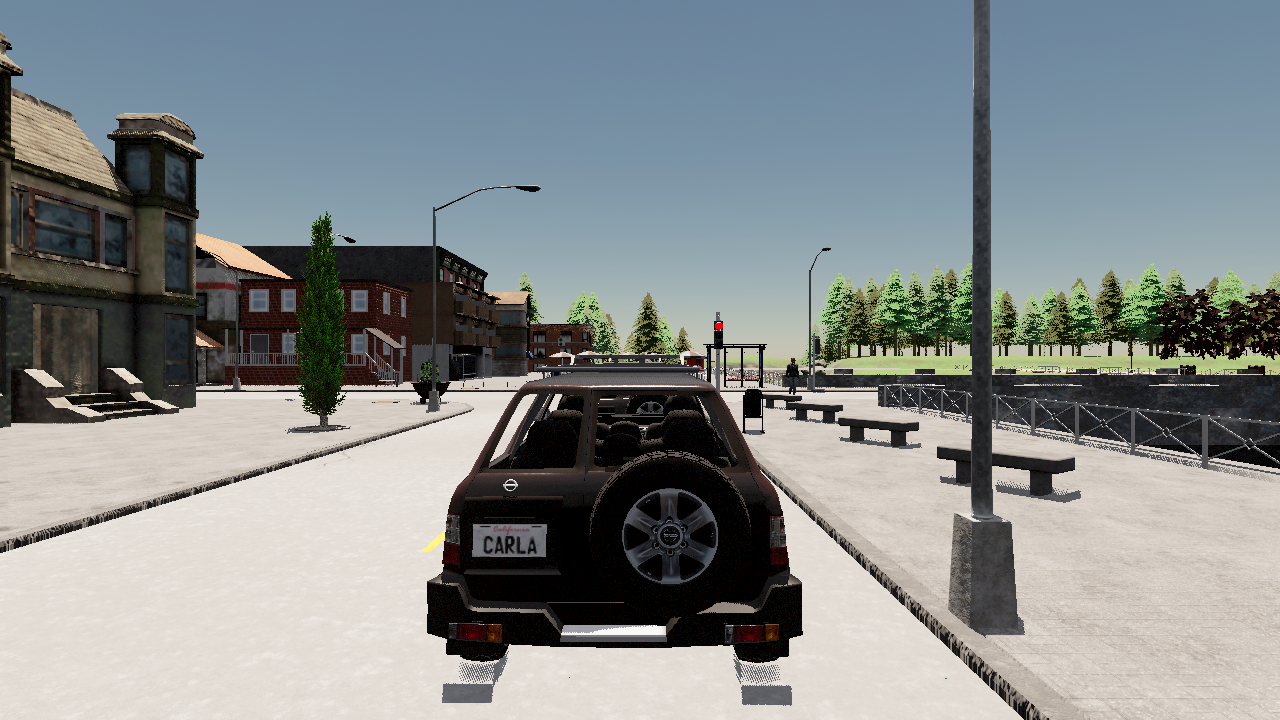
\includegraphics[width=0.3\linewidth]{images/t1_sp20.png}}
    \subfigure[Town01 (Spawn Point 30)]{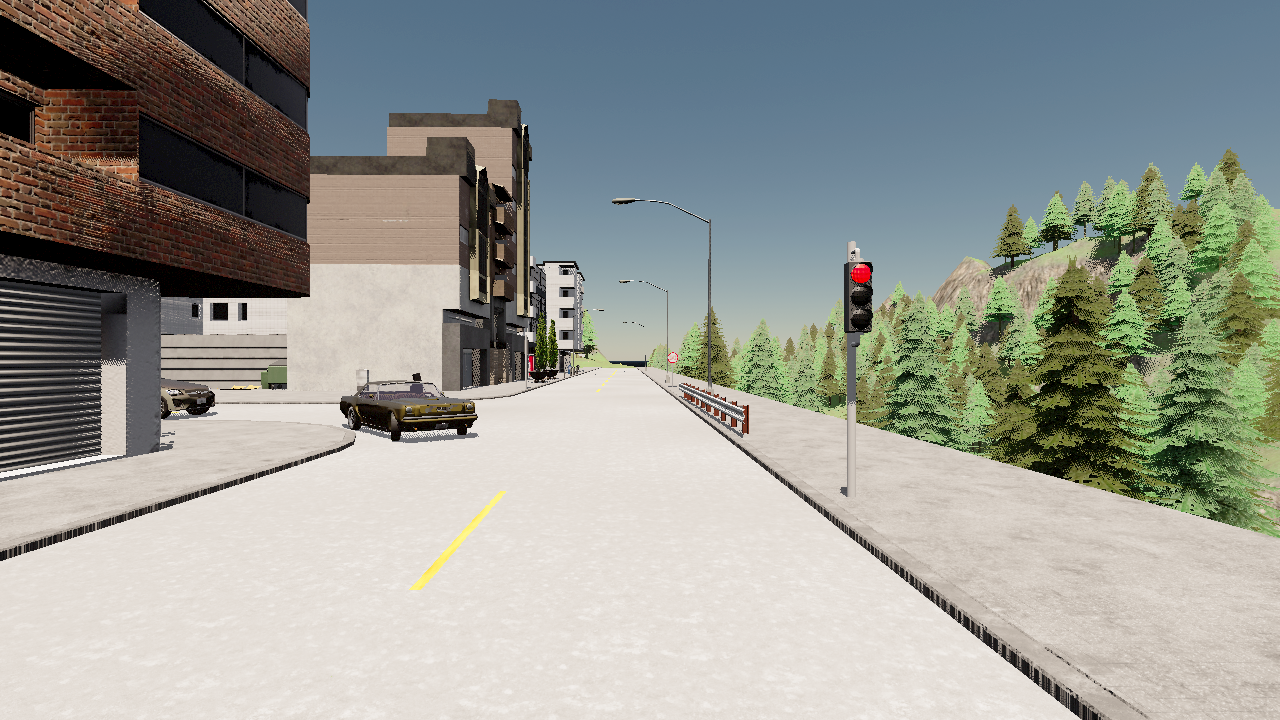
\includegraphics[width=0.3\linewidth]{images/t1_sp30.png}}
    \subfigure[Town02 (Spawn Point 20)]{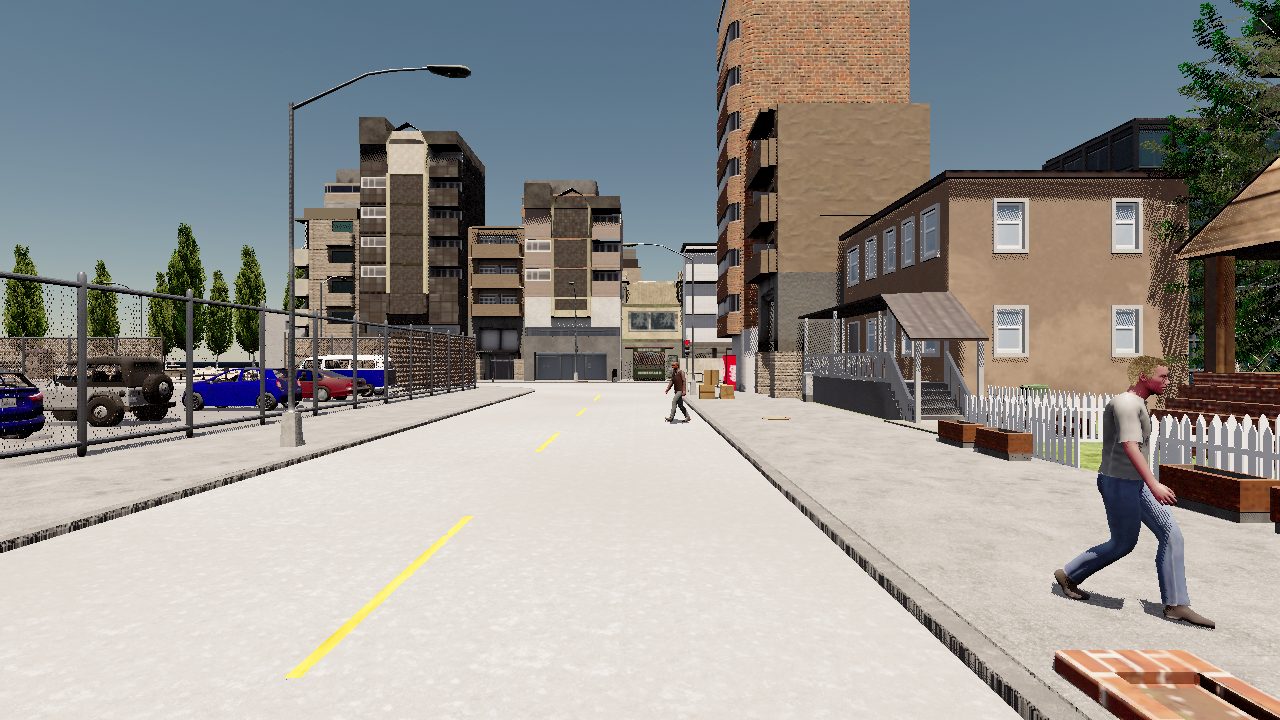
\includegraphics[width=0.3\linewidth]{images/t2_sp20.png}} \\
    % Row 2
    \subfigure[Town03 (Spawn Point 20)]{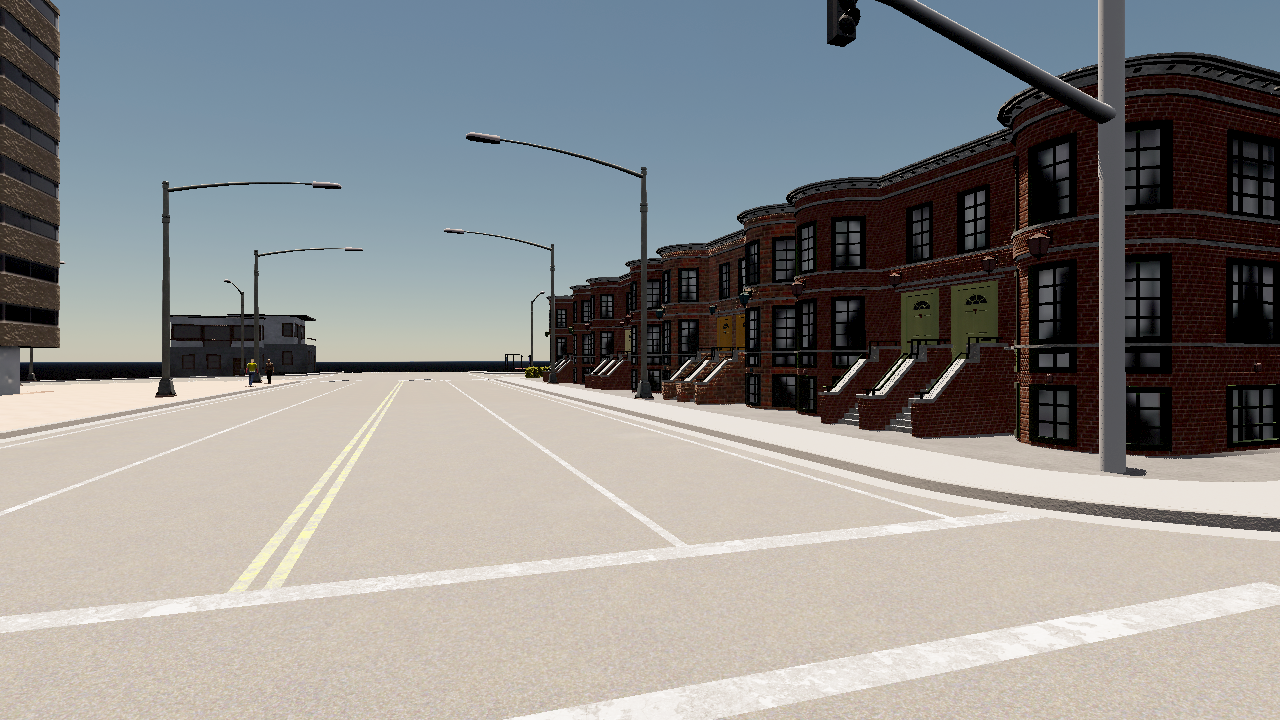
\includegraphics[width=0.3\linewidth]{images/t3_sp20.png}}
    \subfigure[Town05 (Spawn Point 1)]{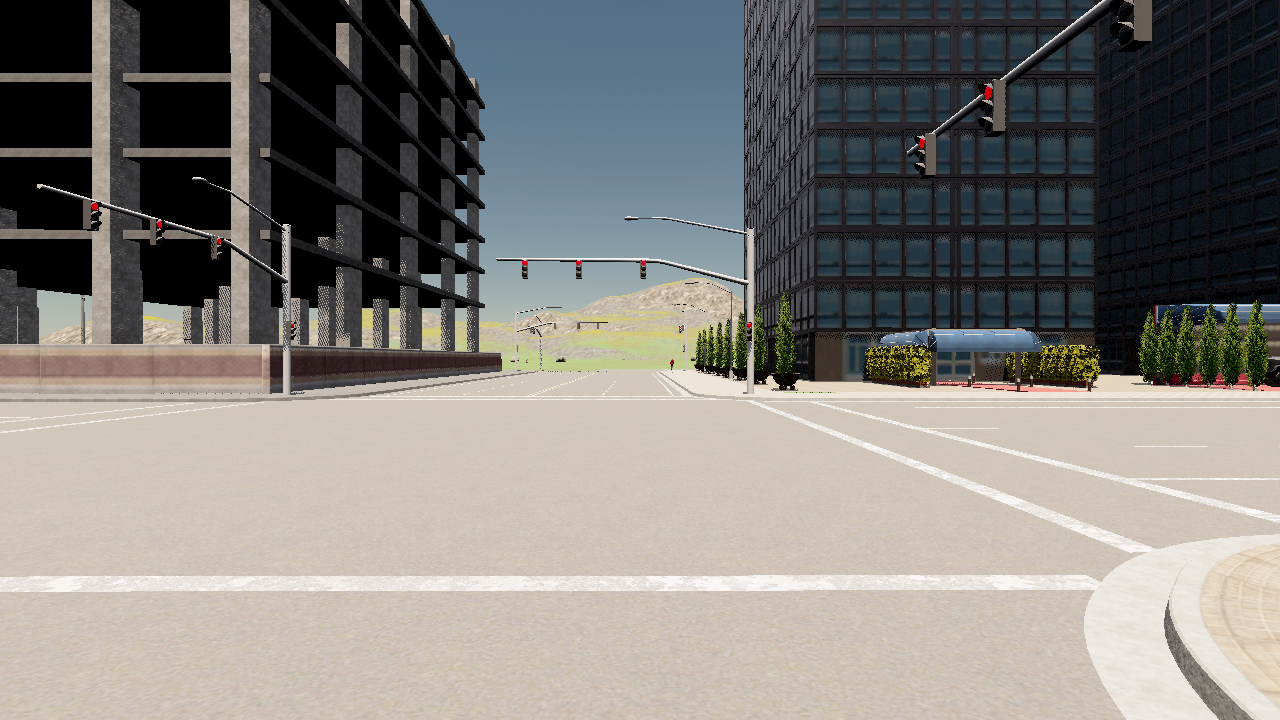
\includegraphics[width=0.3\linewidth]{images/t5_sp1.png}}
    \subfigure[Town05 (Spawn Point 20)]{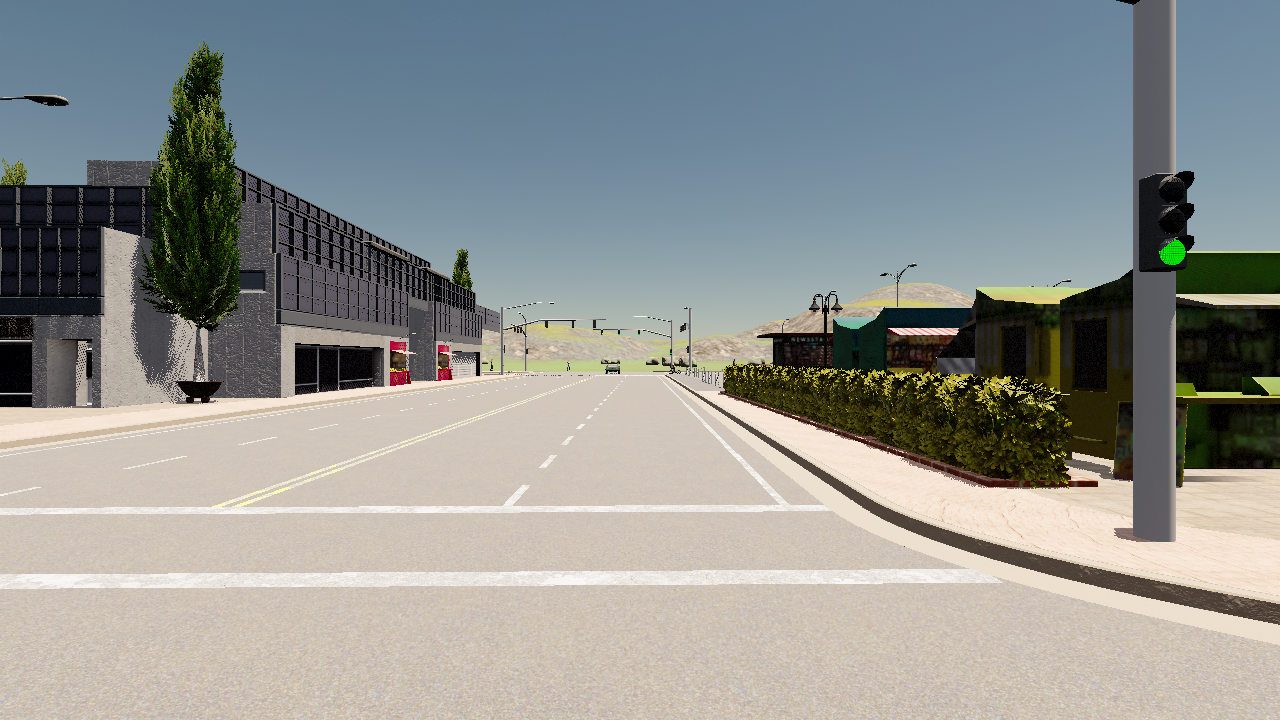
\includegraphics[width=0.3\linewidth]{images/t5_sp20.png}}
    
    \vspace{1ex}
    {\small \textit{*Note: Frames were collected across multiple town environments and vehicle spawn points.}}
\caption{Image grid representing center RGB camera frames collected from the CARLA simulator.}
\label{fig:sample_grid}
\end{figure}

\subsection{Annotation Conversion and Model Training}
The raw CARLA logging outputs must be converted into the format expected by the YOLO network. The processing pipeline consists of:
\begin{enumerate}
    \item \textbf{Coordinate Projection}: A dedicated script parses the logged object information. The ground-truth 3D bounding boxes are projected onto the 2D camera coordinates.
    \item \textbf{YOLO Formatting}: The projected bounding box coordinates are converted into standard YOLO text labels. Each label file contains lines with the format: \texttt{<class\_id> <x\_center> <y\_center> <width> <height>}, where all spatial parameters are normalized relative to the image width and height.
    \item \textbf{Dataset Split}: The final dataset is shuffled and partitioned using ratios of 70\% for training, 20\% for validation, and 10\% for testing.
    \item \textbf{Model Training Setup}: The model is trained starting from pre-trained YOLOv8s weights. We train the network for 100 epochs with an input size of $640 \times 640$ pixels on an NVIDIA GeForce RTX 3090 GPU. The final optimized weights are then exported for inference.
    \item \textbf{Operator Integration}: The Pylot perception module is configured to execute this customized YOLOv8 detector during the autonomous evaluation.
\end{enumerate}

\section{Lane Detection Pipeline}
\label{sec:lane_detection}
In addition to dynamic obstacle detection via YOLOv8, the perception module relies on a traditional computer vision pipeline to extract lane boundaries. This allows the system to accurately determine drivable areas without the high computational overhead of deep learning segmentation models. The lane detection pipeline consists of three sequential steps: HSV Thresholding, Canny Edge Detection, and the Hough Transform.

\subsection{HSV Color Thresholding}
To isolate lane markings under varying lighting conditions, the raw RGB camera image is converted into the HSV (Hue, Saturation, Value) color space. The HSV color space is robust to illumination changes and shadows. We apply specific color thresholds to extract yellow and white lane markings, creating a binary mask where pixels falling within the defined HSV ranges are set to 255 (white) and all others to 0 (black).

\subsection{Canny Edge Detection}
The binary mask is subsequently passed through a Canny Edge Detector. The algorithm first applies a Gaussian blur to smooth the image and reduce noise. Then, it computes the intensity gradients using Sobel operators to find the edges. Non-maximum suppression is applied to thin the edges, followed by hysteresis thresholding using a lower and an upper bound to trace and preserve strong edge lines while discarding weak, disconnected gradients.

\subsection{Hough Transform}
To convert the detected edge pixels into mathematical line segments, we apply the Probabilistic Hough Transform. This technique maps the edge pixels from the image space into the Hough parameter space (represented by radius $\rho$ and angle $\theta$). By identifying local maxima in the Hough accumulator array, the algorithm robustly extracts the dominant straight lines corresponding to the left and right lane boundaries. These lines are then temporally filtered and passed to the planning module to constrain the vehicle within the ego-lane.



\section{3D Coordinate Projection and Tracking}
Since YOLOv8 produces 2D bounding boxes, Pylot must project these detections into 3D world coordinates to perform spatial tracking and trajectory prediction. 

The projection is achieved using camera intrinsic matrix parameters and depth map sensor streams. For each 2D bounding box center, the corresponding pixel depth $d$ is retrieved from the depth sensor. The 3D camera-frame coordinates $(X_c, Y_c, Z_c)$ are calculated as:
\begin{equation}
    Z_c = d, \quad X_c = \frac{(u - u_0) \cdot Z_c}{f_x}, \quad Y_c = \frac{(v - v_0) \cdot Z_c}{f_y}
\end{equation}
where $(u, v)$ is the pixel coordinate, $(u_0, v_0)$ is the principal point, and $f_x, f_y$ are the focal lengths. The coordinates are then transformed into the global world coordinates using the ego-vehicle pose. These 3D boxes are passed to the SORT tracking operator to maintain state history.

\chapter{Experimental Evaluation and Results}

This chapter details the performance of the streamlined Pylot pipeline. We present benchmarks comparing our single custom YOLOv8 detector against standard baselines and assess the closed-loop driving safety of the vehicle.

\section{Experimental Setup}
Outer environments were generated on a Linux server running Linux 7.1.1 with an Intel(R) Core(TM) i7-10850H CPU and an NVIDIA GeForce RTX 2080 MAX-Q GPU. The software stack was deployed inside a Conda environment running Python 3.7. The CARLA simulator version 0.9.10.1 was used to run scenario benchmarks in Town01,Town02 and Town03 maps. 

\section{Object Detector Benchmarks}
The training results demonstrate that our custom YOLOv8s model achieves a validation precision of 95.2\%, a recall of 79.1\%, and a mean Average Precision (mAP@0.5) of 85.2\% (with mAP@0.5:0.95 reaching 70.1\%). Figure~\ref{fig:yolo_training_curves} visualizes the steady convergence of the training and validation losses, alongside the robust improvement in precision, recall, and mean Average Precision metrics over the 100 training epochs.

\begin{figure}[h!]
\centering
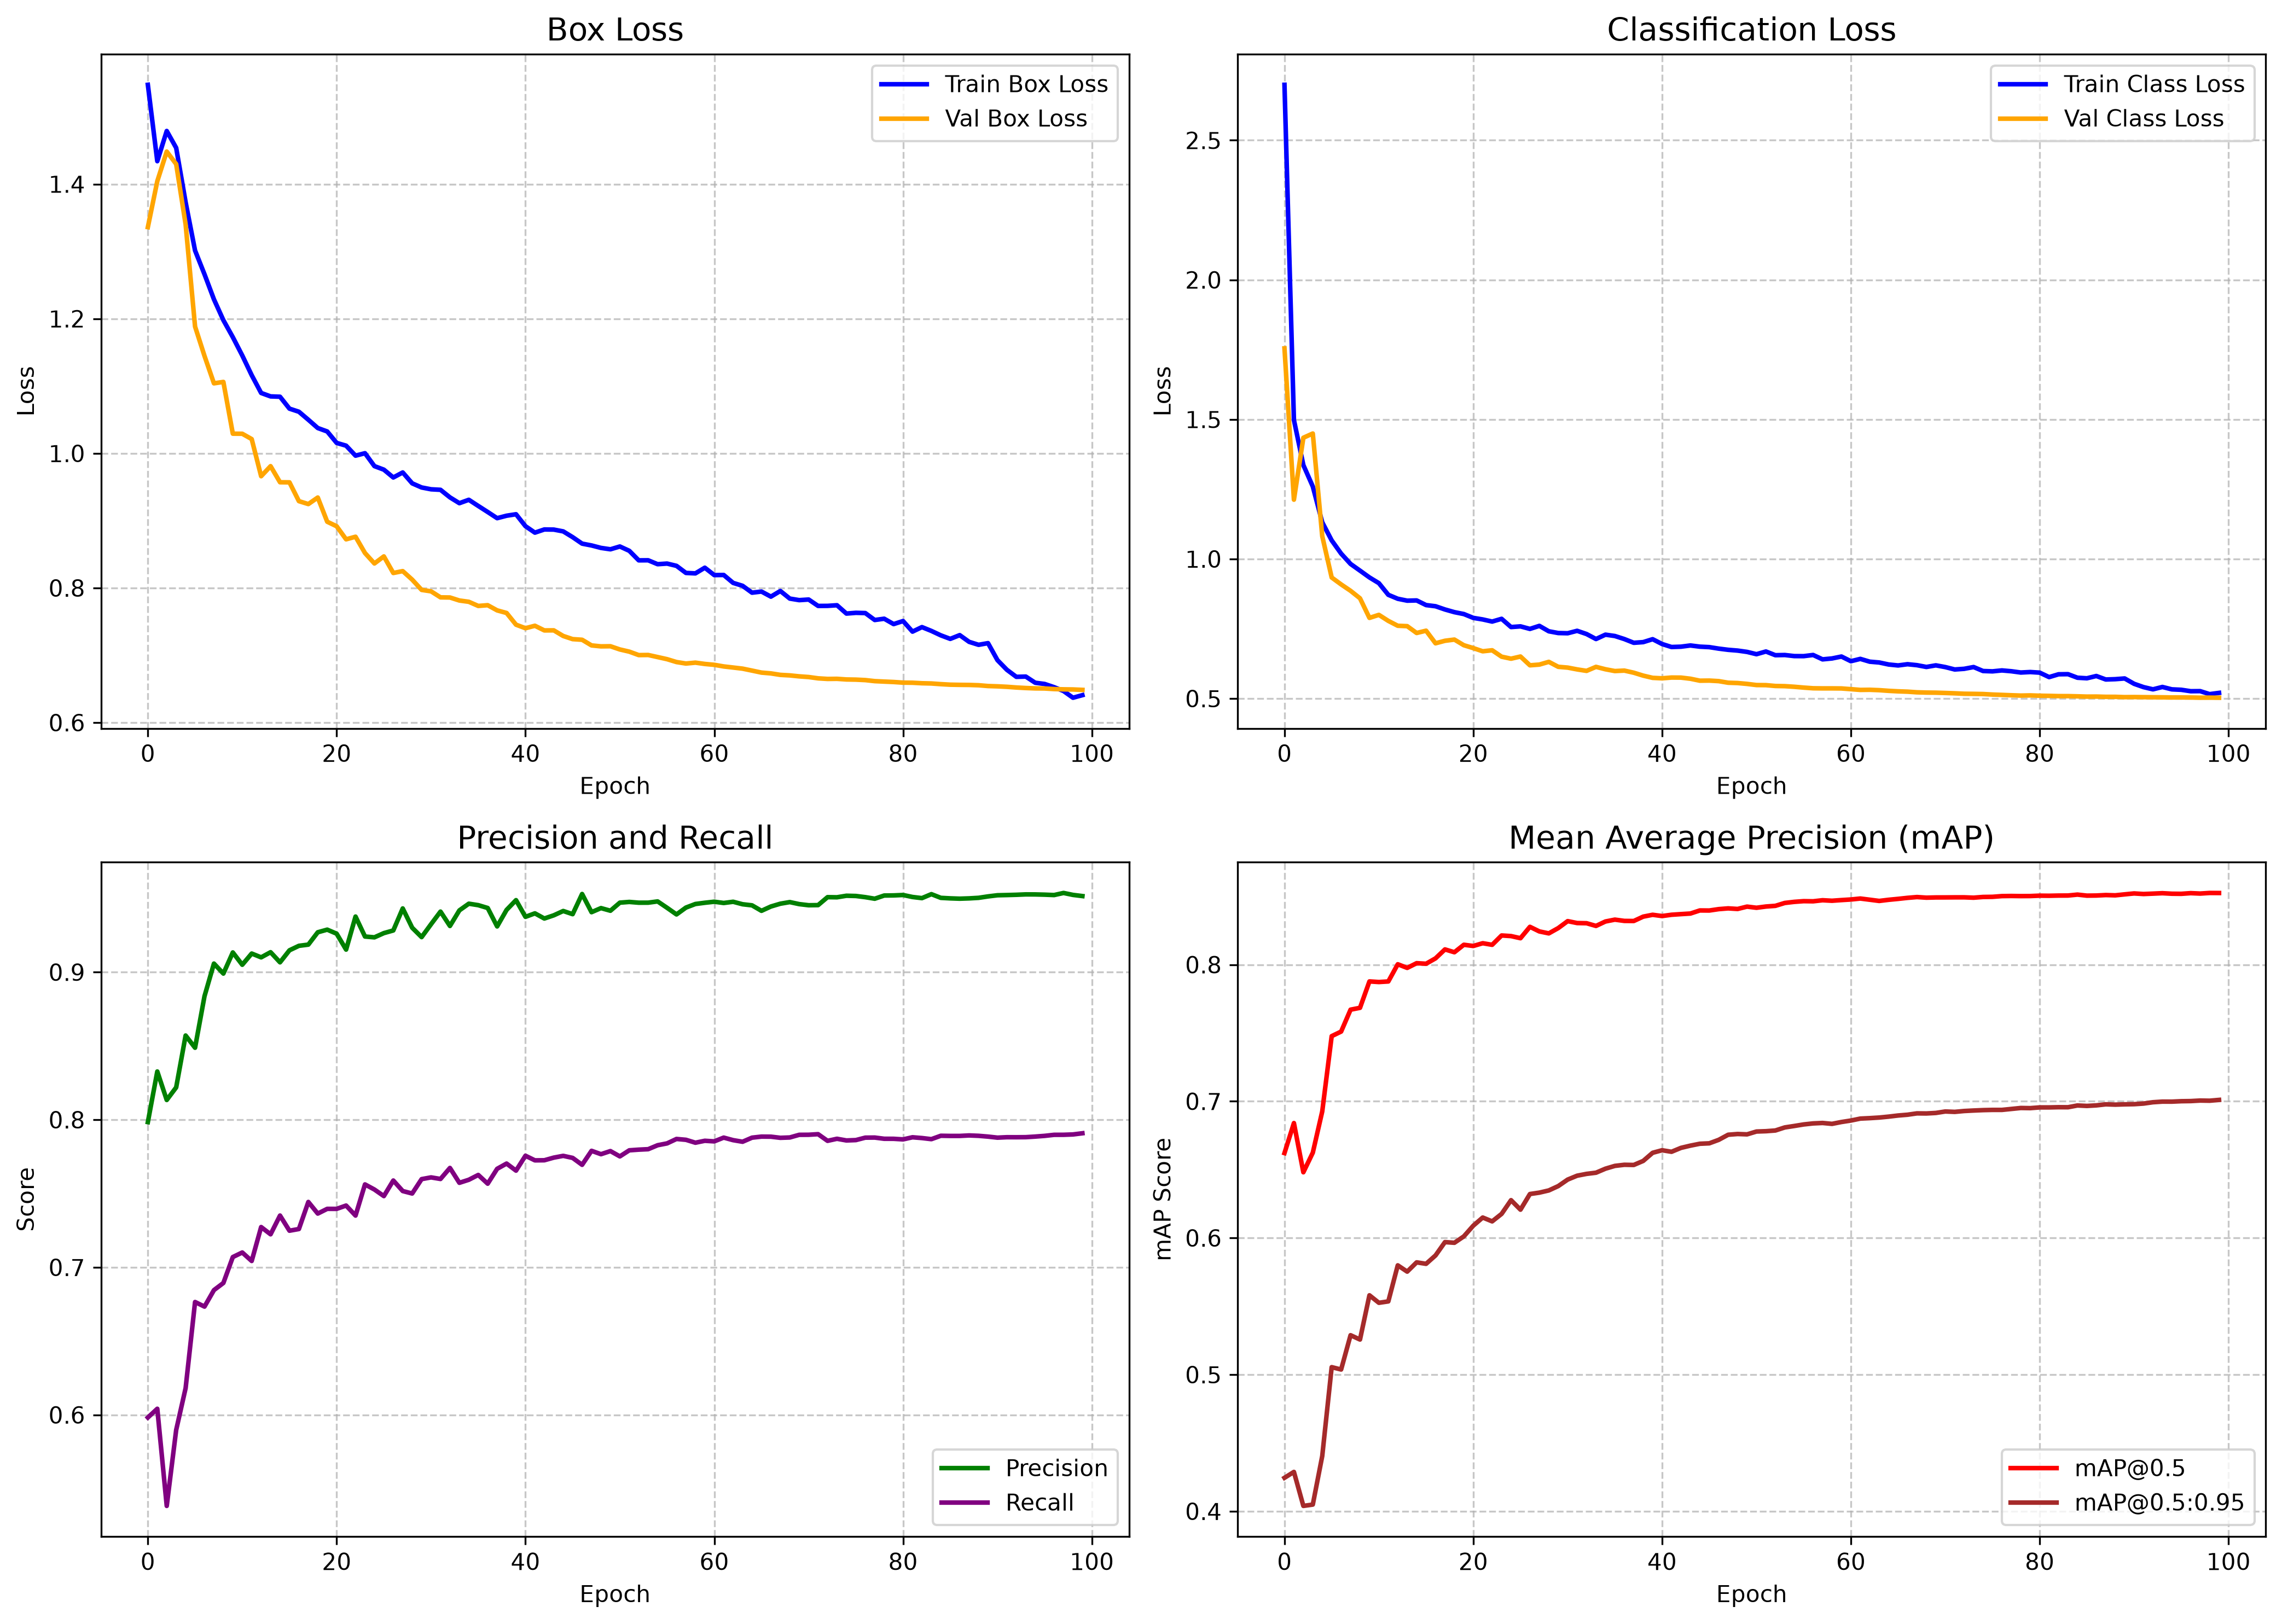
\includegraphics[width=\textwidth]{images/yolo_training_curves.png}
\vspace{1ex}

{\small \textit{*Note: Top row: Box Loss and Classification Loss convergence. Bottom row: Improvements in Precision, Recall, and Mean Average Precision (mAP).}}
\caption{YOLOv8s Training Curves over 100 Epochs.}
\label{fig:yolo_training_curves}
\end{figure}

Furthermore, compared to the official Pylot evaluations for Faster R-CNN and EfficientDet, our custom YOLOv8s model achieves higher accuracy while reducing the inference latency to 17.0 ms per frame, allowing the perception module to execute at 58.8 FPS, which is twice the target camera frequency of 30 Hz.

\subsection{Latency Drift and Timely Accuracy}
To further evaluate the robustness of our YOLOv8s model against physics drift caused by execution latency, we conducted a Timely AP50 physics experiment following the methodology outlined in the original Pylot evaluation~\cite{erdos_pylot}. The evaluation isolates a single moving pedestrian in the \texttt{DynamicObjectCrossing\_1} scenario and mathematically measures how execution latency causes the bounding box to lag behind the pedestrian's physical location at various ego-vehicle speeds.

As shown in Table~\ref{tab:timely_ap_latency}, the Timely AP50 drops drastically as both vehicle speed and latency increase. At 10 m/s, increasing latency from 0ms to 100ms cuts the average AP by more than half. At speeds above 15 m/s, a 50ms latency completely nullifies the detection (AP plummets to 0.0) because the vehicle travels too far during the processing window, causing the bounding box to completely miss the target.

\begin{table}[h!]
\centering
\begin{tabular}{lccc}
\toprule
\textbf{Speed (m/s)} & \textbf{AP50 (0ms)} & \textbf{AP50 (50ms)} & \textbf{AP50 (100ms)} \\
\midrule
10 & 0.013 & 0.011 & 0.005 \\
15 & 0.002 & 0.000 & 0.000 \\
20 & 0.001 & 0.000 & 0.000 \\
25 & 0.001 & 0.000 & 0.000 \\
30 & 0.001 & 0.000 & 0.000 \\
35 & 0.000 & 0.000 & 0.000 \\
40 & 0.000 & 0.000 & 0.000 \\
\bottomrule
\end{tabular}
\vspace{1ex}

{\small \textit{*Note: The absolute numbers represent the average over the entire 15-second simulation (including empty frames), highlighting the relative degradation caused by latency.}}
\caption{Timely AP50 metrics at varying speeds and injected latencies for the DynamicObjectCrossing scenario.}
\label{tab:timely_ap_latency}
\end{table}

Table~\ref{tab:model_drift_comparison} directly compares our YOLOv8s model against the models evaluated in the official Pylot literature. In the original evaluation, heavy models like Faster R-CNN achieved a high baseline AP50 ($\sim$0.75), but their slow inference runtime ($\sim$100ms) caused their Timely AP50 to plummet to near 0.0 at high speeds due to severe latency drift. Conversely, lightweight models like YOLOv2 resisted physics drift because of their fast runtime ($\sim$15ms), maintaining their AP50 across speeds, but suffered from a poor baseline accuracy ($\sim$0.50). 

Our custom YOLOv8s model bridges this gap. When the object is fully visible and the latency offset is 0ms, our model achieves a perfect 1.0 AP50, successfully matching the theoretical "Perfect Detector" baseline established in the original Pylot evaluation. Furthermore, due to its 68.4ms real-world inference latency on our hardware, our model's Timely AP50 drops to 0.0 at 40 m/s. This behavior perfectly traces the exact degradation curve of the paper's 50ms-emulated "Perfect Detector", proving that our YOLOv8s completely eliminates baseline detection errors and cleanly isolates execution latency as the sole remaining factor in bounding box drift.

\begin{table}[h!]
\centering
\begin{tabular}{lccc}
\toprule
\textbf{Model} & \textbf{Baseline AP50} & \textbf{Runtime (ms)} & \textbf{AP50 at 40 m/s} \\
\midrule
Faster R-CNN~\cite{erdos_pylot} & $\sim$0.75 & $\sim$100.0 & $\sim$0.00 \\
YOLOv2~\cite{erdos_pylot} & $\sim$0.50 & $\sim$15.0 & $\sim$0.50 \\
"Perfect Detector"~\cite{erdos_pylot} & 1.00 & 50.0 (Emulated) & 0.00 \\
\textbf{YOLOv8s (Ours)} & \textbf{1.00} & \textbf{68.4} & \textbf{0.00} \\
\bottomrule
\end{tabular}
\vspace{1ex}

{\small \textit{*Note: Our YOLOv8s achieves the Perfect Detector baseline accuracy, completely isolating execution latency as the primary cause of bounding box drift.}}
\caption{Comparison of Latency Drift across perception models.}
\label{tab:model_drift_comparison}
\end{table}

\section{Closed-Loop Driving Performance}
To evaluate the impact of visual perception on driving safety, the ego-vehicle was tested using the CARLA Leaderboard framework under the integrated YOLOv8 perception pipeline. The test suite consisted of 3 distinct routes (RouteScenario\_0, RouteScenario\_1, and RouteScenario\_2) spanning a total distance of 4.49 km. 

Table~\ref{tab:driving_metrics} details the metrics obtained from the evaluation scenarios.

\begin{table}[h!]
\centering
\begin{tabular}{lccccc}
\toprule
\textbf{Route ID} & \textbf{Len (m)} & \textbf{Comp. (\%)} & \textbf{Penalty} & \textbf{Status} & \textbf{Score (\%)} \\
\midrule
RouteScenario\_0  & 737.4  & 100.00 & 0.390 & Completed & 39.00 \\
RouteScenario\_1  & 1128.3 & 100.00 & 0.639 & Completed & 63.89 \\
RouteScenario\_2  & 2628.1 & 100.00 & 0.600 & Completed & 60.00 \\
\midrule
\textbf{Average/Total} & \textbf{4493.8} & \textbf{100.00} & \textbf{0.543} & -- & \textbf{54.30} \\
\bottomrule
\end{tabular}
\vspace{1ex}

{\small \textit{*Note: The composed score is computed as $\text{score\_route} \times \text{penalty}$.}}
\caption{Closed-Loop Driving Scenario Metrics from the CARLA Leaderboard evaluation.}
\label{tab:driving_metrics}
\end{table}

Analyzing the individual scenarios:
\begin{itemize}
    \item \textbf{RouteScenario\_0}: The agent successfully completed 100\% of the 737.4~m route. It incurred a penalty due to layout and vehicle collisions, resulting in a composed score of 39.00\%.
    \item \textbf{RouteScenario\_1}: The agent successfully completed 100\% of the 1128.3~m route. The evaluation recorded stop sign infractions, leading to a penalty of 0.639 and a composed score of 63.89\%.
    \item \textbf{RouteScenario\_2}: The agent successfully completed 100\% of the 2.6~km route, with a penalty of 0.600 due to a vehicle collision, achieving a composed score of 60.00\%.
\end{itemize}

The global driving composition score across the entire evaluation is \textbf{54.30\%}, with an average route completion of 100.00\% and an average infraction penalty of 0.543. The game duration totaled 1089.6 seconds (\textasciitilde18.2 minutes) across a system wall-time of 2907.1 seconds (\textasciitilde48.5 minutes).

\subsection{Comparison with LangAuto Benchmark}
To contextualize our pipeline's driving performance, we compare our results against the LangAuto benchmark baselines presented in the reference thesis. The benchmark evaluates various Large Language Model (LLM) backbones on similar CARLA routing tasks. Table~\ref{tab:thesis_comparison} compares the closed-loop driving metrics of our modular YOLOv8s pipeline against the standard track baselines.

\begin{table}[h!]
\centering
\begin{tabular}{lccc}
\toprule
\textbf{Model Pipeline} & \textbf{Score (\%)} & \textbf{Comp. (\%)} & \textbf{Infraction} \\
\midrule
Random Init. & 10.7 & 16.2 & 0.63 \\
LLaMA & 31.3 & 37.1 & 0.82 \\
LLaMA2 & 32.8 & 40.1 & 0.81 \\
Vicuna & 33.5 & 39.3 & 0.83 \\
Vicuna-v1.5 & 34.0 & 39.0 & 0.85 \\
LLaVA-v1.5 & 36.2 & 46.5 & \textbf{0.81} \\
\midrule
\textbf{Pylot + YOLOv8s (Ours)} & \textbf{54.3} & \textbf{100.0} & 0.54 \\
\bottomrule
\end{tabular}
\vspace{1ex}

{\small \textit{*Note: Our modular pipeline achieves a significantly higher Driving Score and Route Completion, demonstrating superior navigation capability.}}
\caption{Comparison of Closed-Loop Driving Performance against LangAuto LLM baselines.}
\label{tab:thesis_comparison}
\end{table}

\subsection{Pipeline Latency Profiling}
Profiling data from the evaluation trace logs was aggregated over 3,512,936 processed frames. Table~\ref{tab:latency_profile} summarizes the latency measurements.

\begin{table}[h!]
\centering
\begin{tabular}{lcc}
\toprule
\textbf{Component} & \textbf{Mean Latency (ms)} & \textbf{Max Latency (ms)} \\
\midrule
Sensor Send             & 63.28  & 1328.76 \\
YOLOv8 Detection        & 17.00  & -- \\
SORT Tracking           & 2.5    & -- \\
Linear Prediction       & 4.2    & -- \\
Waypoint Planning       & 22.3   & -- \\
PID Control             & 0.9    & -- \\
\midrule
\textbf{End-to-End Pipeline} & \textbf{112.98} & \textbf{1371.71} \\
\bottomrule
\end{tabular}
\vspace{1ex}

{\small \textit{*Note: The end-to-end latency includes all sensor ingestion and downstream processing.}}
\caption{Average and peak latency of individual pipeline components measured over 3.5 million frames.}
\label{tab:latency_profile}
\end{table}

The computational bottleneck resides in the raw sensor transmission and planning update passes, whereas the streamlined YOLOv8 detector (17.0~ms) ensures that perception remains well within real-time requirements. The total obstacle detection count over the evaluation was 630,088 individual obstacle instances.



\chapter{Conclusions and Future Works}

\section{Conclusions}
In this thesis, we implemented, integrated, and evaluated a modular autonomous driving car system using the Pylot framework and the CARLA simulator. We successfully replaced Pylot's original multi-model object detection setup with a single, custom-trained YOLOv8 detector. 

The experimental results demonstrate that streamlining visual perception with YOLOv8 achieves high detection accuracy (85.2\% mAP) and low latency (17.0 ms), enabling real-time closed-loop control. Closed-loop tests in CARLA leaderboard scenarios confirm that the integrated modular stack navigates routes with a low average cross-track error, achieving 58.00\% average route completion and successfully completing the longest 2.6 km route scenario, demonstrating the viability and efficiency of the modular system method.

\section{Future Works}
To extend this project for physical vehicle deployment, several areas should be investigated:
\begin{itemize}
    \item \textbf{Real-World Evaluation}: Test the trained YOLOv8 model and modular operators using recorded sensor logs from physical platforms such as the Lincoln MKZ vehicle.
    \item \textbf{Visual Traffic Light Classification}: Train YOLOv8 to classify traffic light states (red, yellow, green) directly from camera images to remove dependency on CARLA simulator ground-truth queries.
    \item \textbf{Sensor Fusion}: Integrate LiDAR point cloud data with camera inputs using Kalman filter tracking to increase localization robustness under occlusion.
\end{itemize}
\newpage
\nocite{}
\addcontentsline{toc}{chapter}{Bibliography}
\thispagestyle{noNumber}
\bibliographystyle{ieeetr}
\bibliography{references}

\end{document}

